\documentclass[12pt]{article}
%\usepackage[paperwidth=8,paperheight=11cm,textwidth=13cm,textheight=14cm,left=0.5cm,right=0.5cm,top=0.5cm,nohead,nofoot]{geometry} 
%\usepackage[paperwidth=10.1cm,paperheight=13cm,left=0.3cm,right=0.3cm,bottom=0.5cm,top=0.1cm,nohead,nofoot]{geometry} 
\usepackage[paperwidth=10.1cm,paperheight=13cm,left=0.8cm,right=1.2cm,bottom=1.0cm,top=0.1cm,nohead,nofoot]{geometry}

%\usepackage[papersize={4.5in,6in},margin=0.5cm]{geometry}
%\usepackage[body={2cm, 5.5in},left=0.2in,right=0.2in,top=0.2in,bottom=0.2in]{geometry}

\parindent=0cm
\parskip=13pt
% 轉成 PDF 時, 產生 hyperlink 的效果
%\usepackage{CJK}

\usepackage{picinpar}
\usepackage[dvips]{graphicx}
%\usepackage{epstopdf}
\usepackage[dvips]{hyperref}
\usepackage{type1cm}
\usepackage{threeparttable}
\usepackage{fancyvrb}
\usepackage{longtable}

% 在使用 latex2html 可以處理中文
%\usepackage{cwtex}
\usepackage{CJKutf8} %使用CJK套件
\usepackage{comment}
\usepackage{listings}
\usepackage{ucs}

%\setcounter{counter}{10}


%\usepackage[dvips,CJKbookmarks,pdftitle={From TeX/LaTeX to PDF}%
%                ,pdfsubject={From TeX/LaTeX to PDF}%
%		 ,pdfkeywords={tex,latex,cjk,typeset,pdf,typography}]{hyperref}
\usepackage{hyperref} % 最好保证 hyperref 是最后加载的宏包
\hypersetup{%
dvipdfmx,% 设定要使用的 driver 为 dvipdfmx
unicode={true},% 使用 unicode 来编码 PDF 字符串
pdfstartview={FitH},% 文档初始视图为匹配宽度
bookmarksnumbered={true},% 书签附上章节编号
bookmarksopen={true},% 展开书签
pdfborder={0 0 0},% 链接无框
pdftitle={聆听数字的声音}
pdfauthor={李忠},
pdfsubject={sb16},
pdfkeywords={sb16},
pdfcreator={latex},
pdfproducer={PDF 制作程序},% 这个好像没起作用?
}

%\begin{htmlonly}

%\renewcommand{\abstractname}{\r18 摘要}
%\renewcommand{\figurename}{\m11 圖}
%\renewcommand{\contentsname}{\r20 目錄}

%\end{htmlonly}

%\renewcommand{\appendixpagenam}{附錄}
\begin{document}

%\begin{CJK}{UTF8}{bsmi} %開始CJK環境, 設定編碼, 設定字體
\begin{CJK}{UTF8}{gbsn} %開始CJK環境, 設定編碼, 設定字體


% 標題頁
% 正文
\title{聆听数字的声音}
\author{李忠}

\maketitle

\newpage
%\addtocontents{toc}{text}
\tableofcontents
%\addcontentsline{toc}{section}{abstract}
%\addcontentsline{toc}{section}{REFERENCE}
\newpage

\addtocounter{section}{9}
\addtocounter{table}{9}
\addtocounter{figure}{9}
\section{聆听数字的声音}
每次谈到计算机硬件的时候, 人们无一例外地会说总线有多宽, 速度有多快。很难说什么样的“快”才叫快, 特别是考虑到内存和外部设备在速度上和处理器相比, 从来就不在一个数量级上。

数据通常在内存和外部设备之间, 以及一个外部设备和另一个外部设备之间流动。典型的例子包括从硬盘读数据到内存中, 或者从内存中把数据传送到显存中。如果屏幕的分辨率是1280×1024, 在真彩色显示方式下, 每个像素至少需要3个字节。想想看, 以每秒30帧的速度来刷新屏幕上的画面, 这样的事, 也只有现在的技术可以做到, 在从前是不可想象的。现在, 让我们简单快速地回顾一下, 以前是怎样的, 现在又是怎样的。

\subsection{本章意图}
\subsubsection{过气的直接存储器访问}
数据传输毫无疑问地是在总线上进行的, 因为不可能在众多的设备之间建立一对一的连线。但是, 总线的麻烦之处在于如何避免冲突, 当两个家伙对话时, 无关的人都应当关上门闭上嘴。在这种情况下, 必须有一个能够控制总线的设备, 或者称为总线主控设备 (bus master) , 来管理这种事情。

在硬件技术不发达的早期, 处理器是最重要的总线主控制设备, 它有权决定谁参与总线数据传输。考虑以下代码片断:

\begin{verbatim}
mov [0x2000],dx
\end{verbatim}

在执行这条指令时, 处理器不但发出地址信号, 也发出控制信号, 控制信号用来表明该地址是发给内存的, 还是发给外部设备的。所有设备都有译码电路, 这些译码电路的输入就是地址和控制信号。以上指令执行的时候, 内存的译码结果是打开通向总线的数据通路, 而外部设备则保持同总线的脱离状态。
相反地, 下面的指令是发给端口的, 内存当然不会工作。而且, 只有那个端口号相符的外部设备才会和数据总线连通, 其它所有设备都保持同总线的脱离状态:

\begin{verbatim}
in al,0x70
\end{verbatim}

在这种情况下, 如果外部设备希望向内存传输数据, 那么, 必须由处理器首肯并介入其中:
\begin{verbatim}
mov bx,0x2000
mov cx,500
ttime: in al,0x50
mov [bx],al
loop ttime
\end{verbatim}
在这个例子中, 数据先从端口0x50读出, 传送到寄存器AL, 然后再传送到内存单元, 视数据量的大小, 这个过程需要重复多次。
当两个外部设备希望对话时, 比如从一个设备传送200个字节的数据到另一个设备, 情况也差不多:

\begin{verbatim}
mov cx,200
ttime: in al,0x30
out 0x50,al
loop ttime
\end{verbatim}

在过去的岁月中先后出现过多种不同的总线类型, 它们的典型代表就是工业标准结构总线 (Industrial Standard Architecture:ISA) 。总线不单单是数据线路, 还包括地址线路的控制信号线路, 规定和数据和地址的宽度, 以及各种控制信号的规程和电气特性。控制信号规定了设备之间互相交流的协同的方式, 而不同的总线有不同的控制信号规程。

ISA是面向单用户和简单应用环境的总线, 结构并不复杂。所以, 符合ISA信号规程的外部设备都很简单。以今天的眼光看来, 或者以数据传输的效能来看, 对总线的控制能力有限。尽管如此, 它还是提供了一种解决方案, 那就是直接存储器访问 (Direct Memory Access:DMA) 。直接存储器访问的核心器件是DMA控制器 (DMA Controller:DMAC) , 尽管不如处理器那么神通广大, 但也是一个总线主控设备。
一台计算机内只有一个DMA控制器, 由它负责所有外部设备的直接数据传输协调工作, 而且赋予它的总线主控能力要高于处理器。比如, 当外部设备需要发起一次针对内存某个区域的数据传输时, 应该向DMAC发出请求。DMAC回应此请求, 同时告诉处理器不要再使用总线。注意, 这是干预处理器的工作, 命令它让出总线。接着, 由它主导, 开始在该外部设备和内存之间直接传输数据。
如图10-1所示, 在早期的计算机系统中, DMAC是独立于处理器和外部设备之外的第三方 (Thrid party) 总线主控器。设备向DMAC发送DMA请求 (DMA REQuest:DREQ) ;如果总线空闲, 可以占用, DMAC用DMA确认信号 (DMA ACKnology) 回应。此后, 就可以正常开始DMA传送。
 
图10-1  直接存储器访问控制逻辑
\begin{figure}
\begin{center}
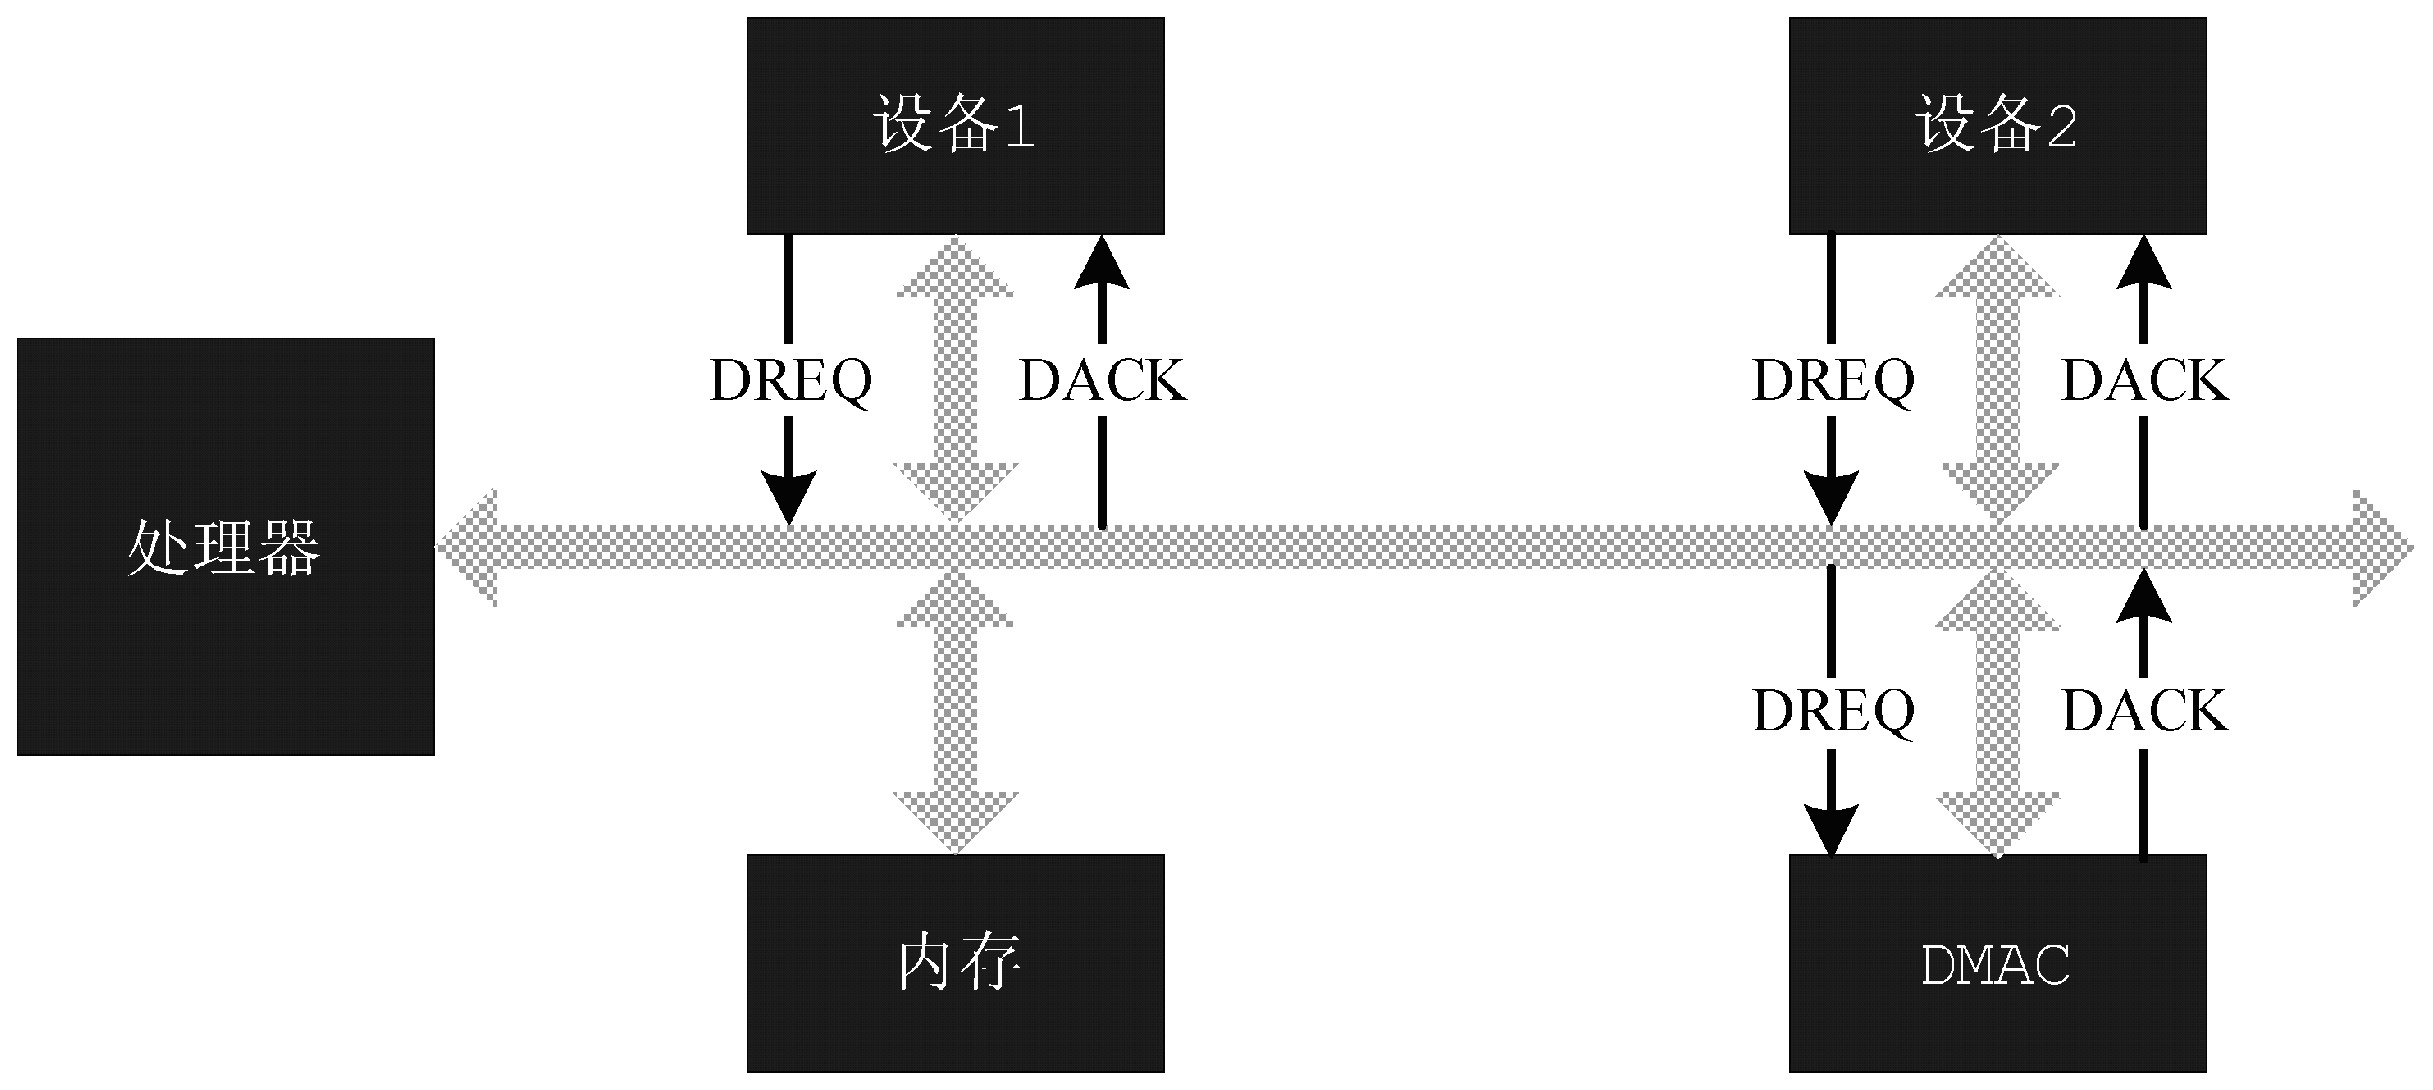
\includegraphics[width=\textwidth]{eps/10-1.bmp.eps}
\caption{直接存储器访问控制逻辑}\label{dma}

%  \begin{adjustbox}{addcode={\begin{minipage}{\width}}{\caption{%
%General-Pupose Instruction}\label{gpinst}
%      \end{minipage}},rotate=90,center}
%      \includegraphics[scale=.6]{eps/instruction_format.eps}%
%  \end{adjustbox}

\end{center}
\end{figure}



对大批量、高速数据传输的需求一直是存在着的, 区别仅仅在于这种需求有多强烈。所谓水涨船高, 要求自然也跟着提高了, 当我们的显卡能够支持高分辨率和真彩色显示模式时, 大家就开始考虑让它能够播放高码率的高清电影。
DMA技术曾经很流行, 但总线技术发展速度更快, 所以, 现在的情况是, DMA技术依然在大学的教材上非常流行, 现实生活中, 在实际的计算机系统中, 它已经渐渐离我们远去。

在个人计算机中, 总线发展的目标是智能、高速和并发地进行输入输出。因此, 为那些有批量数据传输需求的设备提供总线主控能力无疑是非常必要的, 这就是现行的PCI和PCI-E总线所能为我们做的。在这些新型的总线和总线设备上, DMA已经是一个历史名词, 就仿佛它并没有存在过。

不得不说硬件的发展是非常快的, 有很多曾经是主流的硬件慢慢地离我们而去, 包括DMA技术。尽管在现行的ICH芯片中还包括了DMA部件, 但那是看在一些老式设备的面子上留下来的。事实上, 现在已经没有多少老式设备了, 迟早有一天, 这些老家伙, 包括DMA, 都会被清除出去。

\subsubsection{绝迹的Sound Blaster 16声卡}
讲解数据传输技术是很有趣的, 但这需要设计一个典型的例子, 还得结合最新的技术。比如, 我们可以设计一个例子程序, 访问PCI(E)声卡, 用它来播放MP3音乐。在这个过程中, 涉及到MP3文件的解码, 这会让我们接触到处理器的多媒体指令;也涉及到PCI(E)声卡的数据传输控制, 这会让我们见识如何访问PCI(E)设备, 以及对它们编程的一般方法;数据的传输是处理器、声卡和应用程序三方参与的事情, 这还涉及到彼此的通信和协调, 这能让我们了解到中断机制是如何发挥作用的。

这真是一个复杂的例子, 并不适合目前的学习进度, 因此只能放在下册来做。现在, 比较实际的做法是先打一个简单的基础, 看一看DMA是怎么工作的。在本章, 我们同样会写一个声音播放程序, 但是, 用到的硬件都非常古老, 除了DMA, 还有曾经的Sound Blaster 16声卡, 这种声卡已经绝迹了。

Sound Blaster的发音听起来很像“嗓子拨拉得疼”, 所以又叫声霸卡就不值得奇怪了, 毕竟都是谐音。Sound Blaster 16简称为SB-16, 是新加坡创新公司的杰出产品, 当年一统江湖, 名气很大。不像显卡, 现在的显卡还能同以往保持兼容, 所以我们的程序还能工作, 但声卡不同, 现在的声卡都不能按Sound Blaster 16的方式工作。所以, 本章的程序只能在虚拟机上运行, 在真实的计算机上, 是发不出任何声音的。

Virtual Box虚拟机中有声卡类型选项, 甚至可以选择“Bound Blaster 16”, 但是很明显, 那是个虚拟的硬件。虚拟机会把你针对硬件的访问和操作转化成对真实声卡的访问。所以, 这意味着, 要想用本章的程序播放出声音来, 宿主机, 也就是安装虚拟机的真实机器, 必须是有声卡和扬声器的。

启动Virtual Box, 选择你创建的虚拟机 (比如LEARN-ASM) , 单击“设置”, 进入参数设置对话框。如图10-2所示, 选择“声音”项目。
 
图10-2  为虚拟机设置声卡类型
\begin{figure}
\begin{center}
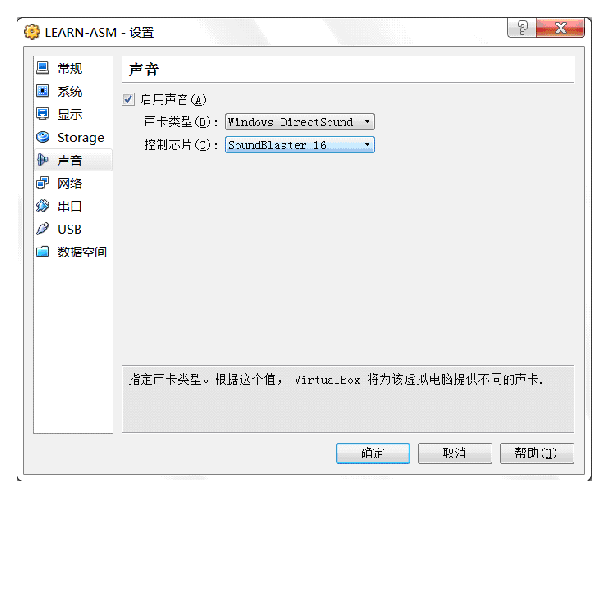
\includegraphics[width=\textwidth]{eps/10-2.bmp.eps}
\caption{为虚拟机设置声卡类型}\label{vm}
\end{center}
\end{figure}

首先要选择 ``启动声音''。然后, 选择声卡类型为 ``Windows DirectSound''。该选项的意思是, 当你在虚拟机里针对声卡硬件进行操作时, 虚拟机也会访问真实的物理声卡来做转换工作, 而虚拟机访问物理声卡的方式是调用Windows操作系统的DirectSound驱动程序。除了我们, 现在谁还会直接针对硬件编程?

顺便说一句, DirectSound是DirectX的一部分, 而DirectX解决了电子游戏程序在Windows上运行时慢如蜗牛的问题, 它为游戏程序提供了一种绕过Windows图形用户接口的工具和方法, 允许它们直接访问显卡和显存。开发这套工具的三个核心人物, 是微软公司内部的讨厌鬼。那家伙们有着令人愤恨的怪僻, 经常脚步沉重地提着一把塑料战斧穿过走廊, 跟人说话的姿势夸张得好像正从自己的头脑中拿出一点智慧施舍给对方。他们在微软帝国高层毫不知情的情况下开发出这套多媒体接口, 开创了游戏行业的新天地。

“控制芯片”的意思是, 你采用什么声卡。声卡有自己的微处理器, 即I/O处理器, 通常称为数字信号处理器 (Digital Singal Processor:DSP) 。习惯上, 人们喜欢用声卡芯片的型号来指代声卡的型号。这里, 应当选择“Sound Blaster 16”。谢天谢地, 尽管有很多虚拟机可供选择, 但能够支持Sound Blaster 16的并不多, Virtual Box虚拟机算是其中的一个。

\subsubsection{代码清单}
%\lstinputlisting[basicstyle=\footnotesize, frame=single,frameround=tttt,breaklines=true,title=modify a little version,escapeinside=``]{c10.asm}
%\lstinputlisting[basicstyle=\footnotesize, breaklines=true,title=代码清单,extendedchars=true]{c10.asm}

10-1
\VerbatimInput[fontfamily=tt,fontsize=\scriptsize,frame=lines, framerule=0.4mm, numbers=left, numbersep=2pt, tabsize=2]{c10.asm}
%\verbatiminput[numbers=left]{c10.asm}

\subsection{声卡和声卡的初始化}
\subsubsection{Sound Blaster 16声卡简介}
声卡是数字和声音的转换器件, 录音的时候, 声波可以推动磁场中的线圈, 也可以使处于静电场中的两个电极间距改变, 或者使碳精砂的疏密程度发生变化, 又或者使压电陶瓷振动, 从而产生音频电流。

音频电流是模拟信号 (Analog Signal) , 模拟信号是连续变化的信号, 就像水流, 强度和大小可以变化, 但这种变化是一种渐变。例如, 当你关断水龙头的时候, 它是逐渐从有到无的, 不失连续性。

如图10-3所示, 这是一个模拟信号, 假设它是从话筒传过来的音频电流。显然, 它是随时间连续变化的, 时间的单位是毫秒 (ms) ;变化的幅度用电压来表示, 这里的单位是毫伏 (mv) 。
 
\begin{figure}
\begin{center}
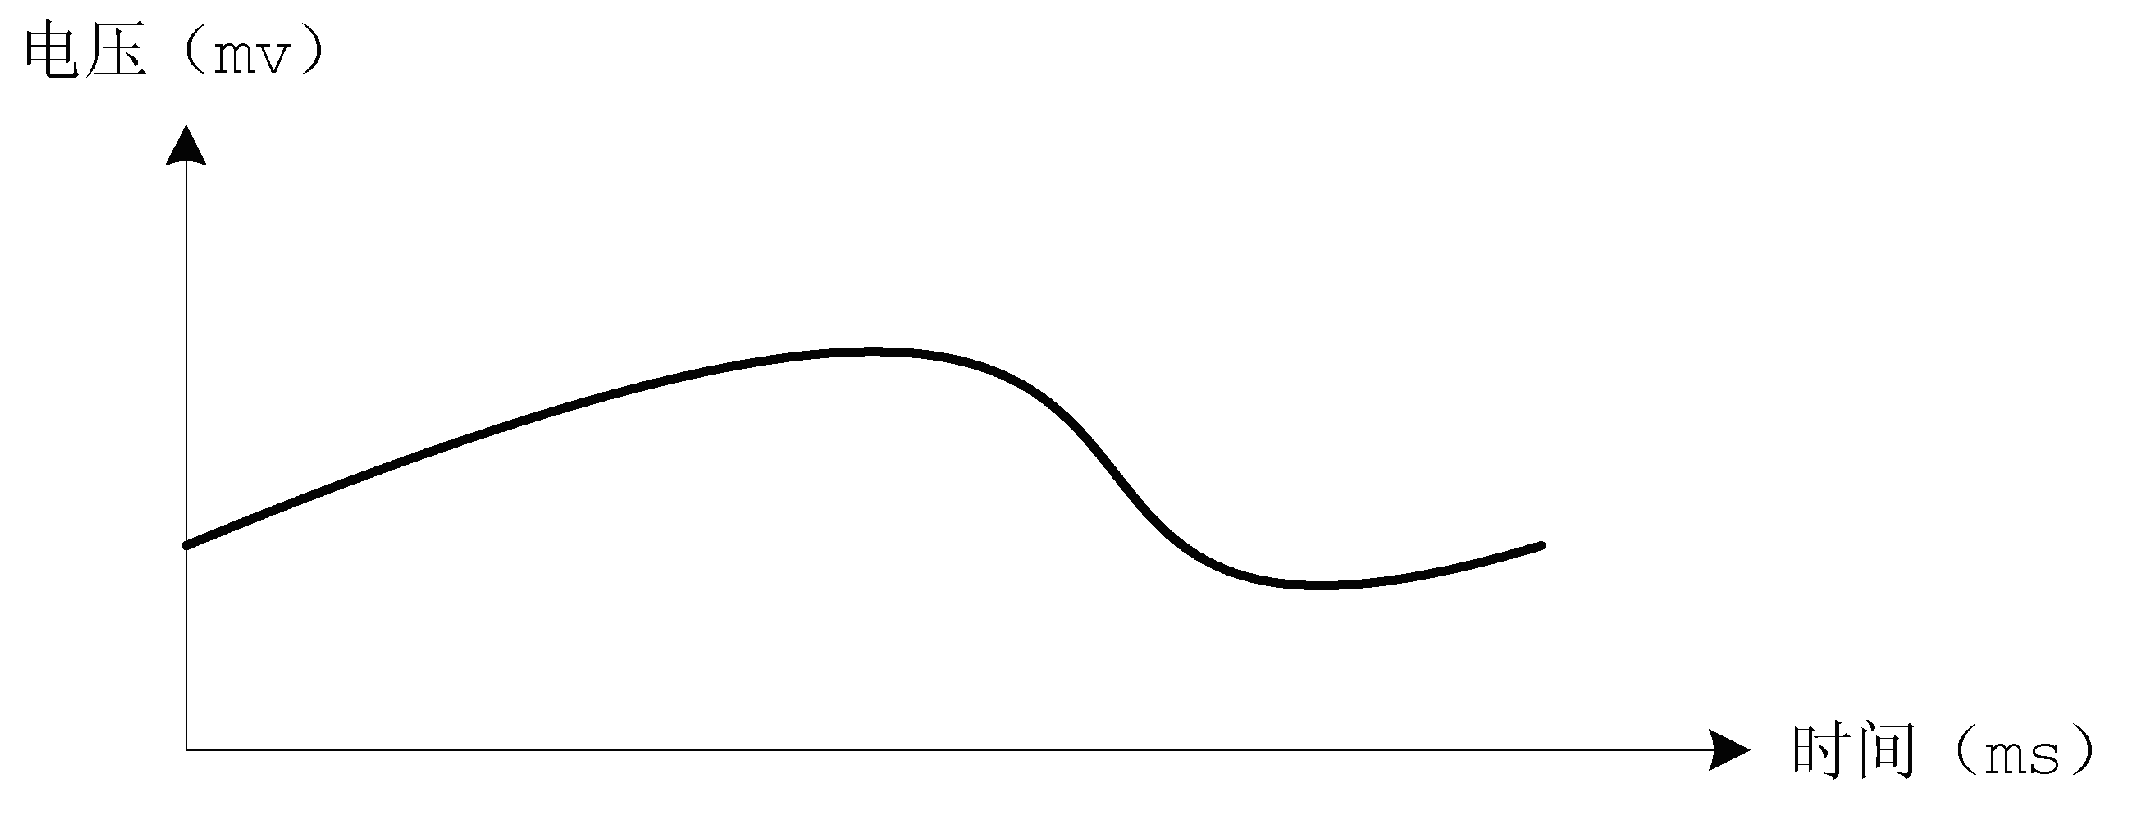
\includegraphics[width=\textwidth]{eps/10-3.bmp.eps}
\end{center}
\caption{随时间变化的模拟信号}
\end{figure}
%图10-3  随时间变化的模拟信号

和模拟电子器件不同, 电子计算机使用的是数字信号 (Digital Signal) 。要使计算机能够处理和保存声音, 必须先进行数字化 (Digitization) , 这涉及到模-数转换, 也就是把模拟信号转换成数字信号。

模-数转换的知识在《穿越计算机的迷雾》这本书里介绍得很详细, 但不妨在这里重温一下, 其中最关键的地方是定时对模拟信号进行观察, 并记录它的幅度 (比如电压的数值) , 这个过程称为采样 (Sampling) 。很显然, 采样的频度决定了是否能真实反应模拟信号的变化情况, 我们通常所说的CD品质, 其典型的采样率是每秒种44100次。另外, 样品的等级也很重要, 使用8位二进制数来记录采样的数值, 只能生成256个等级的样本;使用16位二进制数, 则可以有65536个等级。显然, 位数越多, 精度越高。

Sound Blaster 16 声卡支持双声道 (立体声)、每声道 16 位样本、最高 44.1
KHz的采样和回放。传统上, 要访问该声卡, 需要通过4个端口, 每个端口的功能如表 \ref{sb-16} (p \pageref{sb-16})
所示。

%表10-1 SB-16 端口一览表
\begin{threeparttable}
\caption{SB-16 端口一览表}\label{sb-16}
\begin{tabular}{p{2.7cm}p{1.5cm}p{2.5cm}}
\hline
功能 & 端口号 & 说明 \\
\hline
声卡复位 &	0x226 (只写) & 	将声卡复位到默认工作状态 \\
\hline
读数据	& 0x22A (只读)& 	从声卡读数据 \\
\hline
写命令/数据	& 0x22C (读/写) &	向声卡发送命令或者数据 \\
\hline
W 缓冲区状态\tnote{*} & 0x22C (读/写) &	指示声卡是否已经准备好接受命令或者数据 \\
\hline
R 缓冲区状态\tnote{!}& 0x22E (只读) 	& 指示是否可从声卡接受数据 \\
\hline
\end{tabular}
\begin{tablenotes}\small
\item[*]W 缓冲区用来接受外部的命令和数据。
\item[!]R 缓冲区用来存放供外部读取的数据。
\end{tablenotes}
\end{threeparttable}
%注:W缓冲区用来接受外部的命令和数据;R缓冲区用来存放供外部读取的数据。

\subsubsection{初始化声卡的DSP芯片}
代码清单10-1的总体结构和第八章、第九章的用户程序一样。最主要的, 程序头部是一模一样的, 符合我们自己定义的标准。
代码清单10-1的入口点在第81行, 从第82行到87行, 用于初始化各个段寄存器, 使它们指向相应的逻辑段, 这和以前的章节是一样的。

第89~90行, 用于显示字符串, 表明当前正在初始化声卡设备。字符串是在后面的数据段定义的。字符串显示例程put\_{}string位于当前代码段内, 是从第22行开始定义的, 一直到第45行结束。和前面的做法不同, 这里直接用的是BIOS中断int 0x10的第0x0e号功能。

该过程首先将用到的相关寄存器压栈保护, 然后从给定的缓冲区内把字符一个一个地取出, 并调用BIOS中断予以显示。当取到的字符是0x00时, 表明遇到了字符串的结尾, 于是恢复相关寄存器内容, 返回主过程。注意, 这段代码经历了好几次修改, 最开始的时候, 在过程put\_{}string内部, 并不是采用BIOS中断来显示字符, 所以调用它的时候, 都使用寄存器BX来传递字符串的偏移地址。最后, 当确定要在put\_{}string内部使用BIOS中断的时候, 寄存器BL却要用来传递字符显示属性。在这种情况下, 为了不修改那些调用put\_{}string例程的代码, 让它们依然采用BX来传递地址, 只能修改put\_{}string过程, 在它的内部, 第29行, 把BX的内容传送到SI, 使用SI来寻址要显示的字符。
接着回到代码清单10-1, 现在的工作是初始化声卡, 使它处于默认的工作状态, 就好比掌柜的在每次算帐前都晃一下算盘, 使每个珠子都回到原位一样。初始化SB-16需要三个步骤:
\begin{enumerate}
\item 向0x226号端口写数字0x01, 并等待3毫秒;
\item 向0x226号端口写数字0x00;
\item 典型的 SB-16 声卡需要 100 毫秒来初始化自己。在此期间, 可以不停地读取
0x22e 号端口, 并判断数据的最高位 (第 7 位) 是否为``1''。如果是比特 ``1'', 表明可以从
0x22a 端口读取声卡的状态。如果从 0x22a 号端口返回的内容是 0xAA, 表明声卡已经准备就绪。否则,
意味着声卡没有安装, 或者端口号不正确。
\end{enumerate}
为此, 第93~95行用于向0x226号端口写数字1;第97~100行采用一个循环来进行延时。该延时并不精确, 它只是将寄存器AX清零, 然后减一 (此时的值为0xFFFF) , 接着判断是否为零, 不为零则继续将AX减一判断。在65536次循环之后, 延时结束。
第102行, 向同一端口写数字0。由于在延时后, 寄存器AX的内容为零, 故直接将AL中的内容写入端口0x226。在进行到这一步之后, 软件应当读0x22e端口, 如果第7位是“1”, 再读0x22a端口, 判断是否为0xaa。从声卡读取工作状态的步骤都一样, 可能以后还会做这样的事, 为此, 专门定义了一个过程read\_{}dsp。

过程read\_{}dsp位于代码清单10-1的第65行, 结束于第78行。第69~72行是一个循环, 反复从0x22e端口读一个字节, 直到发现其第7位变成“1”。然后, 第73~78行, 从0x22a端口读取状态字节, 并返回。
回到主程序, 在调用过程read\_{}dsp之后, 第105行, 判断刚才读取的状态字节是否为0xaa。如果不是, 则显示错误信息后转移到程序结尾, 进入停机状态;如果声卡复位正常, 则转移到第112行接着执行。

\subsection{声卡中断}
\subsubsection{中断和声音播放的关系}

你可能很难理解中断和声音播放之间会有什么联系。事实上, 在绝大多数时候, 要播放声音, 中断是必不可少的一环。
播放声音是采样的逆过程, 是连续地将数字转换成模拟信号。同时, 将得到模拟信号放大, 用来推动扬声器, 我们就听到还原后的声音了。可以想象, 这些数字信号都是原先采样得到的, 现在只是回过头来重新播放, 这也许就是称为“回放” (Playback) 的原因吧。

为了回放声音, 最容易想到的办法是连续不断地向声卡传送数字, 直到把所有的数字都传完, 这称为直接模式 (Direct Mode) 。事实上, 这恰恰是最麻烦的做法。回放的难点不在于数-模转换, 这个电路很简单。真正的难点在于如何把握回放的速度, 也就是要精确地控制采样率。

SB-16只支持8位单声道的直接模式。更为遗憾的是, 速率的控制是用户程序的事, 声卡不为此负责。所以, 你可能需要对计算机系统中的定时器芯片编程, 使它定时发出中断信号。不要把定时器芯片和RTC芯片混淆, 它们是两样东西。定时器芯片可以是具有悠久历史 (也就二十多年吧) 的8254, 也可以是用来代替8254的高精度事件定时器 (High Precision Event Timer:HPET) 。

定时器应当按采样率所要求的间隔定期发出中断信号, 每次中断发生时, 就往声卡发送一个数字。在直接模式下, 采样率没有上限和下限, 仅仅取决于定时器中断的频率和中断处理程序的效率。至于回放效果, 据很多人说, 不太好听。而且, 说是直接模式, 其实对于处理器、声卡和人来说, 都直接是个负担。

和直接模式不同, SB-16允许多种能自动控制数据传输的回放模式, 但都需要DMA机制, 而且同样需要中断。当声卡开始回放时, 它会向DMAC发出直接存储器传输请求, 在得到允许后, 占用总线, 从内存中获取数据并自动按设置的采样率进行回放。

像显卡和声卡这种东西都是很贪婪的恶霸, 当它们工作的时候, 每秒钟都要产生或者消耗大量的数据。一首3分钟的歌曲, 一般会有15MB的数据量, 经过压缩之后, 可能会有3MB。即使是经过了压缩, 在播放之前, 依然需要在内存中还原。

无论如何, 内存是有限的, 通常要由声音回放程序提供一小块内存, 称为缓冲区。声音数据通常以文件的形式存放在硬盘和光盘上, 在回放的时候, 才一点一点地读到缓冲区, 再从缓冲区传输到声卡。假设缓冲区的大小是8KB, 那么, 在回放之前, 先填满这块缓冲区, 同时, 设置声卡, 告诉它, 每当读取的数据达到4KB的时候, 发出一个中断信号。

当中断发生的时候, 中断处理程序要判断, 是不是所有的数据都传送完毕。如果是, 就向声卡发送结束回放的命令;如果不是, 则继续用新的数据填充刚刚被声卡用过的那4KB区域。这样一来, 当声卡正在播放的时候, 下一个4KB的数据已经准备好了, 从而不致于使声音中断。

\subsubsection{在声音播放中使用中断}
为了播放声音, 我们在当前代码段内定义了中断处理程序dsp\_{}interrupt, 是从代码清单10-1第224行开始的。该中断处理过程是怎么工作的, 后面就要讲到, 现在的任务是将其安装到中断向量表中。

代码清单10-1第117~118行, 在屏幕上显示一条消息, 说是要安装中断了, 云云。如图 \ref{sb16-8259} 所示, 传统上, SB-16声卡是连在8259主片的第5个中断输入引脚IR5上的。在计算机启动期间, BIOS程序会初始化8259, 将主片的中断号定义成从0x08开始, 所以IR5对应的中断号是0x0d。

\begin{figure}
\begin{center}
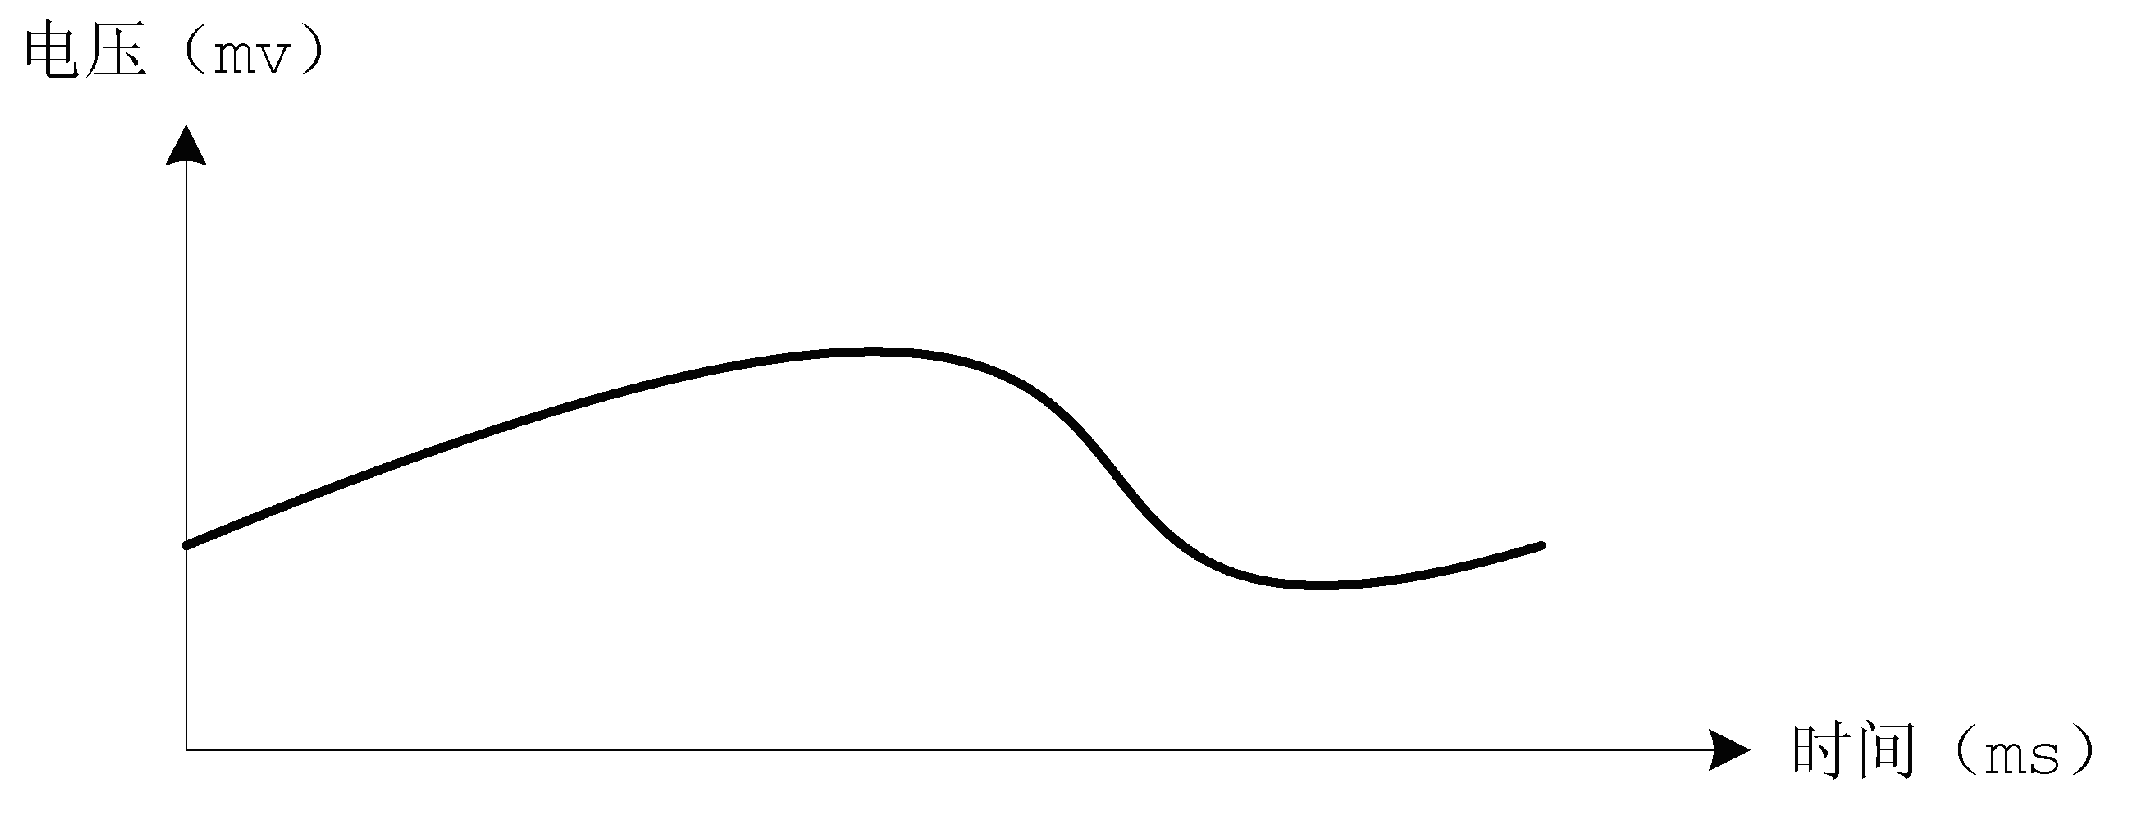
\includegraphics[width=\textwidth]{eps/10-4.bmp.eps}
\caption{从SB-16到8259主片的连接}\label{sb16-8259}
\end{center}
\end{figure}
%图10-4  从SB-16到8259主片的连接

第120~123行, 和以前一样, 把中断号乘以4, 就得到了它在中断向量表中的登记项。事实上, 因为将一个二进制数逻辑左移2次就相当于乘以4, 所以这几句等效于

\begin{verbatim}
mov bx,0x0d
shl bx,2
\end{verbatim}

不过, 这样一来, 指令的功能和意图就显得不是那么明显了。

第125行, 在修改中断向量表的时候, 要禁止外部中断。

第127~137行, 先将段寄存器ES压栈保存, 再使它指向逻辑段0x0000, 这是中断向量表所在的段。接着, 用新的段地址和偏移地址修改0x0d号中断的登记项。0x0d号中断所在的登记项, 其偏移地址已经位于寄存器BX中;新的0x0d号中断处理过程位于当前代码段, 段地址自然由段寄存器CS提供, 偏移地址就是标号dsp\_{}interrupt的汇编地址。当然, 最后还要从堆栈中恢复段寄存器ES的内容。
第137行, 开放外部中断。

既然中断处理过程的入口地址已经安装停当, 第140~142行, 修改8259主片的中断屏蔽寄存器, 使其第5位为“0”, 意思是允许中断信号进入, 同时保持其它位不变。这几句执行之后, 来自声卡的中断请求将会被8259接受。
第144~145行, 显示一条信息, 提示中断处理过程已经安装好了。

\subsection{DMA控制器的结构、功能和初始化}
\subsubsection{个人计算机中的DMA控制器}
如图 \ref{isa_bus} 所示, 在二十年前, 个人计算机系统的组成大致就是这个样子。那个时候, 已经有了集成外围芯片, 内部集成了8259、RTC/CMOS RAM、DMA控制器、定时器/计数器、串/并行通信器、键盘控制器等, 但并不如现在的ICH智能。
 
\begin{figure}
\begin{center}
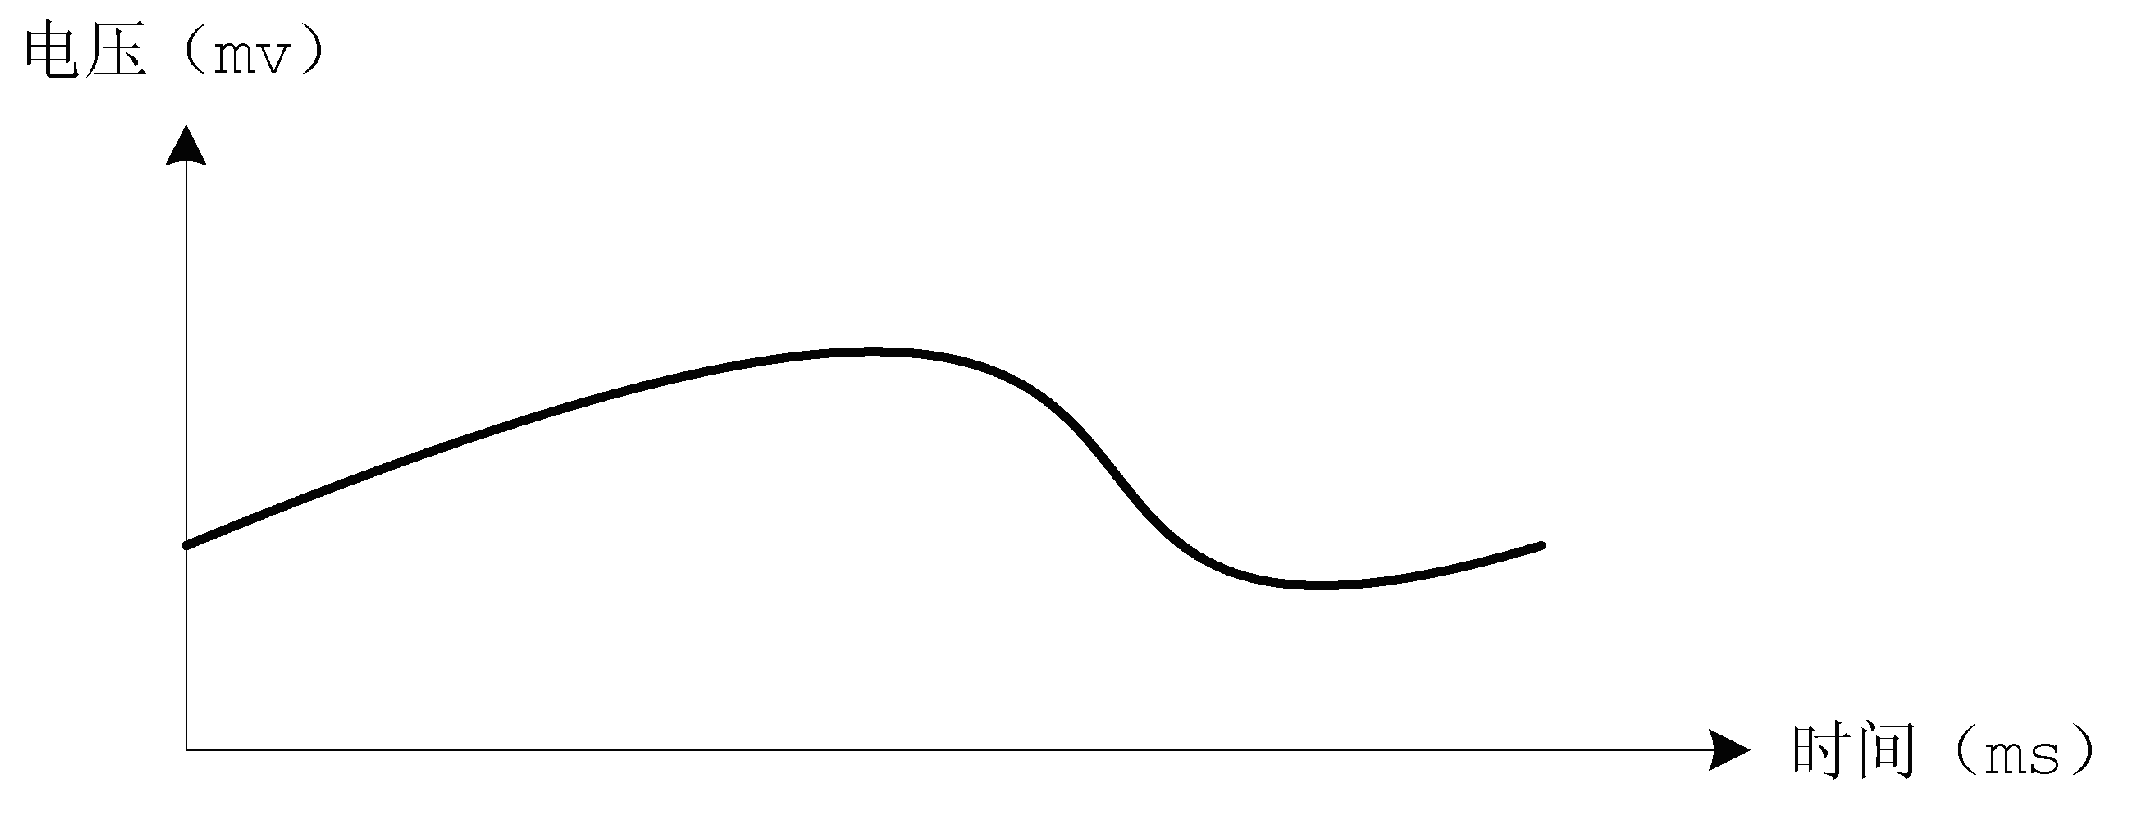
\includegraphics[width=\textwidth]{eps/10-5.bmp.eps}
\caption{ISA 总线、声卡、中断和 DMAC}\label{isa_bus}
\end{center}
\end{figure}
%图10-5  ISA总线、声卡、中断和DMAC

那个时候流行的是ISA总线, 声霸卡就插在ISA总线的扩展槽上。所有这些设备都通过总线和处理器通信, 软件通过I/O端口就可以访问和控制它们。

如图10-6所示, 在当时, DMA芯片用的是8237, 每片4个DMA通道, 可以为4个设备提供DMA请求服务。请求保持信号 (Hold ReQuest:HRQ) 和处理器连接, 请求处理器让出总线, 并在传送期间保持不变。
个人计算机系统通常使用两片8237芯片, 它们通过级联的形式提供7个DMA通道。如图所示, 从片的通道请求引脚和主片的HRQ引脚相连。历史上, SB-16和主片上的通道1相连。
 
\begin{figure}
\begin{center}
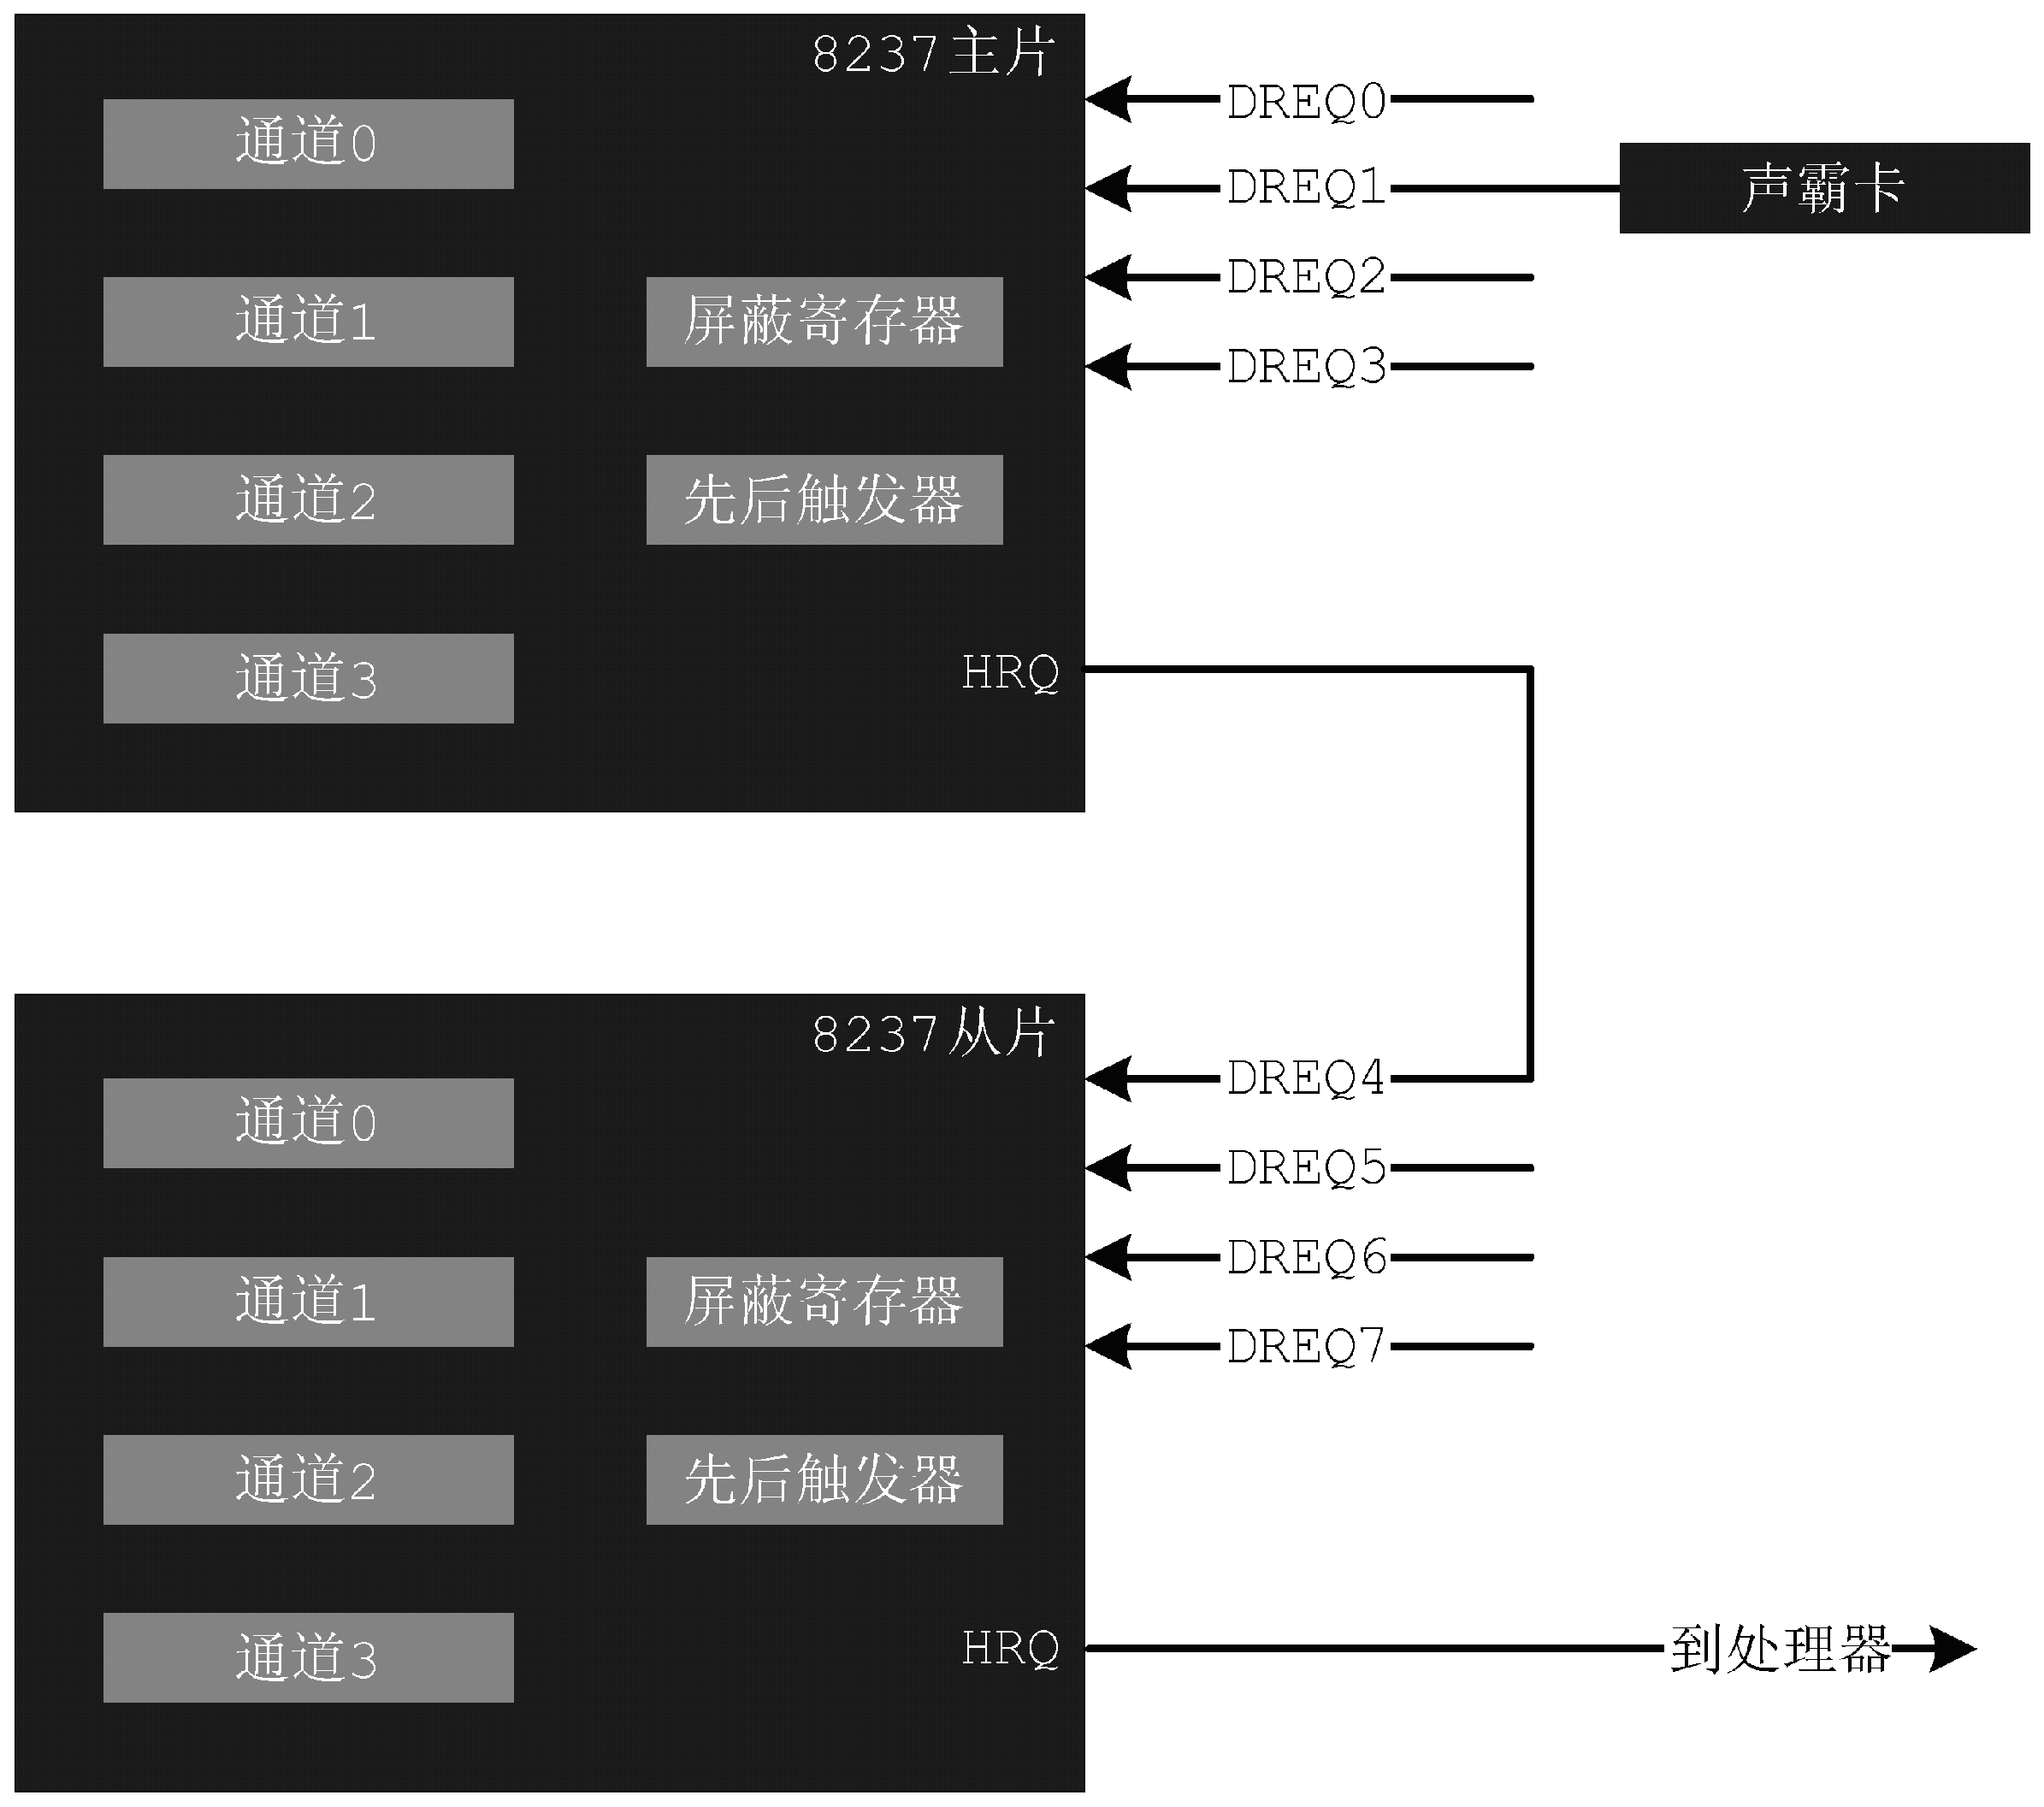
\includegraphics[width=\textwidth]{eps/10-6.bmp.eps}
\caption{个人计算机系统中的 DMA 控制器}\label{dma}
\end{center}
\end{figure}
%图10-6  个人计算机系统中的DMA控制器

尽管ISA总线已经退役, PCI(E)总线大行其道, Sound Blaster 16声卡也已经销声匿迹, 但它所使用的端口号依然留着。而且, 在现在的ICH内部, 依然集成有两片DMA控制芯片, 分别叫做82C37A, 留着它们仅仅是照顾老软件和老硬件的需求。
不用感到疑惑, 本章的程序可以在当今流行的单处理器计算机上工作, 除了缺少一个真实的SB-16声卡。在这样的计算机系统中, 仍然有8259A和82C37A芯片, 虚拟机所做的, 就是虚拟出一个声卡来, 并把它映射到传统的端口上。所以, 只有这一部分是假的。

\subsubsection{初始化DMA控制器 (伪指令incbin) }
每一片82C37A芯片都有个各通道公用的屏蔽寄存器, 用来允许或者关断外部DMA请求信号, 每个通道都可以单独设置。屏蔽寄存器在主片上的端口号是0x0a;在从片上的端口号是0xd4。

为了设置和初始化DMA控制器, 需要先关闭相应的DMA通道, 以免在此期间受到DMA请求信号的打扰。SB-16声卡使用主片上的通道1, 现在就来关闭该通道。

代码清单10-1第151行, 指定将对0x0a号端口进行读写, 这是个8位端口, 只能写入, 不能读出, 对应着主片上的屏蔽寄存器。
第152~153行, 向指定的端口写屏蔽命令, 屏蔽命令的格式如图 \ref{named} 所示。当前指令的意图是关闭主片上的通道1。
 
\begin{figure}
\begin{center}
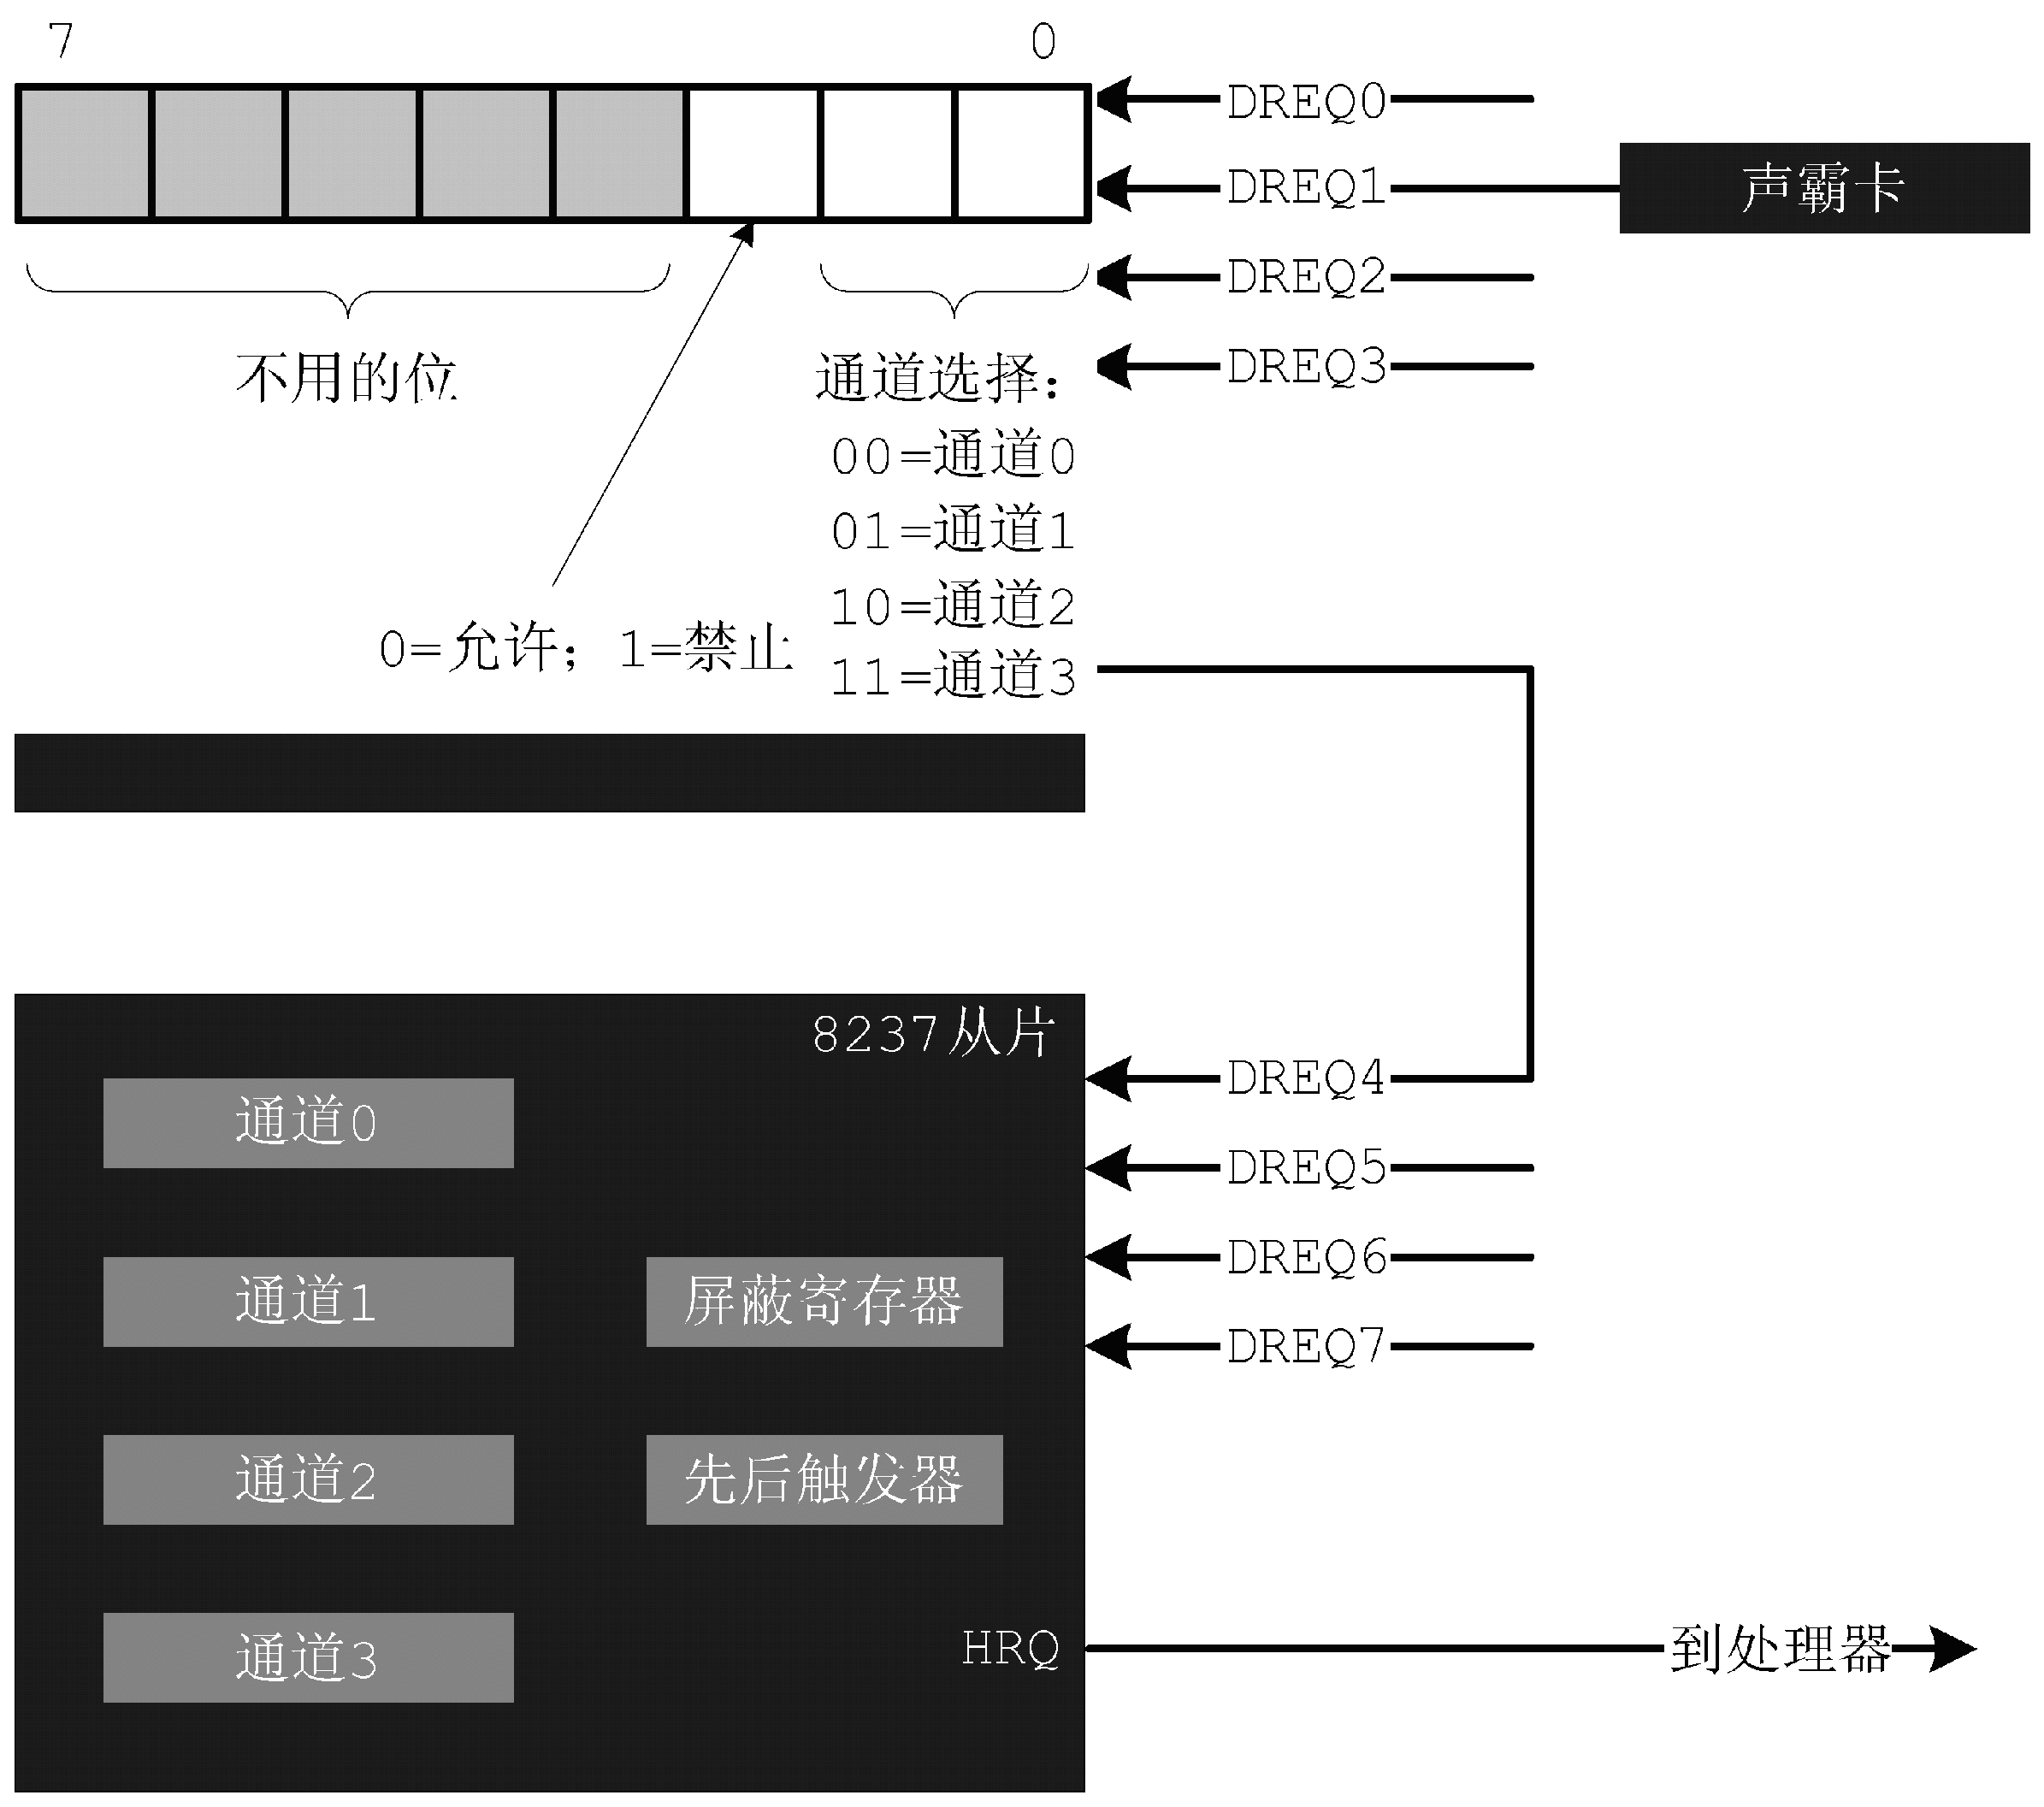
\includegraphics[width=\textwidth]{eps/10-7.bmp.eps}
\caption{通道屏蔽命令的格式}\label{named}
\end{center}
\end{figure}
%图10-7  通道屏蔽命令的格式

82C37A芯片的功能像是在紫禁城里指挥宫女们种菜消遣的慈禧太后, 同时也像个遥控器, 也许都不像。通常来说, 谁需要从内存中读数据, 谁就负责给出地址。但是你看, 在DMA传送过程中, Sound Blaster 16声卡需要数据, 但却不知道数据在哪里, 也不负责给出地址, 给出地址的是82C37A芯片。内存倒还好说, 它只需要地址和内存读写命令, 并把数据放到数据总线上, 从来也不管这些信号来自哪里, 由谁接收。

在82C37A内部, 每个通道都有自己的基准地址寄存器和当前地址寄存器。在DMA传送开始前, 这两个寄存器的内容应当由软件设置成相同的值, 都指向数据在内存中的起始物理地址或者末端物理地址。具体是起始物理地址还是末端物理地址, 取决于是正向传送还是反向传送。
当前地址寄存器的作用是在DMA传送的过程中提供物理地址。在传送的过程中, 每传送一个字节, 当前地址寄存器自动加一或者减一, 以指向下一个数据所在的位置, 而基准地址寄存器的内容始终不变。

数据在内存中所占用的区域通常称为缓冲区 (buffer) , 根据需要, 可大可小, 但应当始终保持不变, 它的起始物理地址或者末端物理地址就是要设置到基准地址寄存器和当前地址寄存器的数值。俗话说“铁打的营盘流水的兵”, 内存空间从来都是有限的, 缓冲区可以定义得小一点, 数据量大的时候, 可以分批进行。比如说, 声音文件位于硬盘上, 大小是64KB, 可以在内存中定义2KB的缓冲区, 每次从硬盘上读取512个字节到缓冲区, 再从缓冲区通过DMA传送到声卡, 共分32个批次。

在这种情况下, 每个批次都要重新设置82C37A芯片的当前地址寄存器, 使它重新指向缓冲区的起始物理地址或者末端物理地址, 这显然很麻烦。为此, 82C37A支持自动预置模式, 如果允许这种模式, 那么, 每当一个批次的数据传送完毕之后, 它会自动用基准地址寄存器的内容来初始化当前地址寄存器, 这就是基准地址寄存器的作用。

那么, 怎样才算是达到了一个批次的传送呢?答案是, 每个DMA通道都有自己的基准字数寄存器和当前字数寄存器。在DMA传送开始前, 软件应当把它们设置成相同的内容。当DMA传送开始时, 每传送一个字节, 当前字数寄存器的内容减一, 而基准字数寄存器的内容始终不变。如果当前字数寄存器的内容为零, 就说明一个批次传送完毕, 82C37A芯片会产生一个传送过程结束的信号。同时, 如果允许自动预置功能, 82C37A就会重新把基准字数寄存器的内容写入当前字数寄存器。

缓冲区是必须准备一个的, 而且, 原则上, 我们应当分批次将声音数据从硬盘上读入缓冲区, 并传送到声卡进行回放。但是, 为了简单起见, 我们特意将声音数据直接包含到用户程序中, 并将它看成是缓冲区。不同之处仅仅在于, 这个缓冲区用不着分批次刷新。
在本章中, 提供的声音文件是baby.wav, 和本章的源代码文件放在同一个目录下, 该文件的大小是57.3KB, 几乎是一个逻辑段的长度 (64KB) 。这是有意的, 因为在实模式下, 段的长度不能超过64KB, 而我们又想直接将它放在程序中的数据段中, 作为一个静态的缓冲区使用。使用超过64KB的大文件是完全可以的, 但不能直接将它包含在编译后的二进制文件中, 最好的办法是存储到硬盘上的其它区域, 并分批从硬盘上读取和播放。考虑到代码的长度和复杂性, 这样的工作还是留给你在业余时间研究吧。

现在, 接着回到代码清单10-1中, 数据段data是在第257行定义的 (使用了vstart=0子句) 。在该段中, 声明了标号voice\_{}data并初始化了一块静态数据, 使用的是伪指令incbin。

incbin的意思是包含外部的二进制文件 (INCluding external BINary files) , 它的功能是将指定的文件逐字地包含到编译后的结果中, 从它在源程序中出现的位置开始。通常, 它可以在游戏程序中直接包含图像和声音数据。
incbin的后面需要三个参数, 第一个参数是文件名。举个例子:

\begin{verbatim}
incbin “baby.wav”
\end{verbatim}

这将会把baby.wav文件的内容原样包含进最终的编译结果中去。

再比如:

\begin{verbatim}
incbin “baby.wav”,44
\end{verbatim}

这句的意思是, 在编译的结果中包含baby.wav文件的内容, 但跳过该文件开头的40个字节。
如果该伪指令的后面出现有三个参数, 比如

\begin{verbatim}
incbin “baby.wav”,44,50000
\end{verbatim}

那么, 编译器将会在编译结果中包含baby.wav文件的内容, 但跳过该文件开头的44个字节, 而且实际上仅仅包含50000个字节。
因此, 在第259行, 程序中使用了incbin伪指令包含声音文件baby.wav, 并且跳过开头的44个字节。wav文件是Windows音频文件, 它的前44个字节是文件头, 其内容如表10-2所示。

%表10-2  Windows波形文件文件头格式
\begin{longtable}{p{1.7cm}p{1.1cm}p{4.8cm}}
\caption{Windows波形文件文件头格式}\label{win_wave} \\
\hline
文件头内部偏移	& 长度 (byte) 	& 含    义\\
\hline
0x00 & 4 & 字符串“RIFF”\\
\hline
0x04 & 4 & 文件长度\\
\hline
0x08 & 4 & 字符串“WAVE”\\
\hline
0x0c & 4 & 字符串“fmt ”, 该串表明这里是音频格式部分的开始\\
\hline
0x10 & 4 & 音频格式部分的长度\\
\hline
0x14 & 2 & 编码格式 (0x01:PCM) \\
\hline
0x16 & 2 & 声道数量\\
\hline
0x18 & 4 & 采样率 (样本生成速度, 即, 采样次数/秒) \\
\hline
0x1c & 4 & 数据率 (采样或回放时, 每秒的字节数) \\
\hline
0x20 & 2 & 数据块大小 (样本宽度/8 ×声道数) \\
\hline
0x22 & 2 & 样本宽度 (8、16或者32, 指每个样本的比特数) \\
\hline
0x24 & 4 & 字符串“data”, 该串表明这里是音频数据部分的开始\\
\hline
0x28 & 4 & 实际的数字音频数据长度 \\
\hline
\end{longtable}

讲述wav文件的文件头格式时, 结合一个实际的例子可能是个好主意。好吧, 让我们来看看本书中用到的baby.wav。用配书工具hexview打开它, 显示的内容如图10-8所示。
 
\begin{figure}
\begin{center}
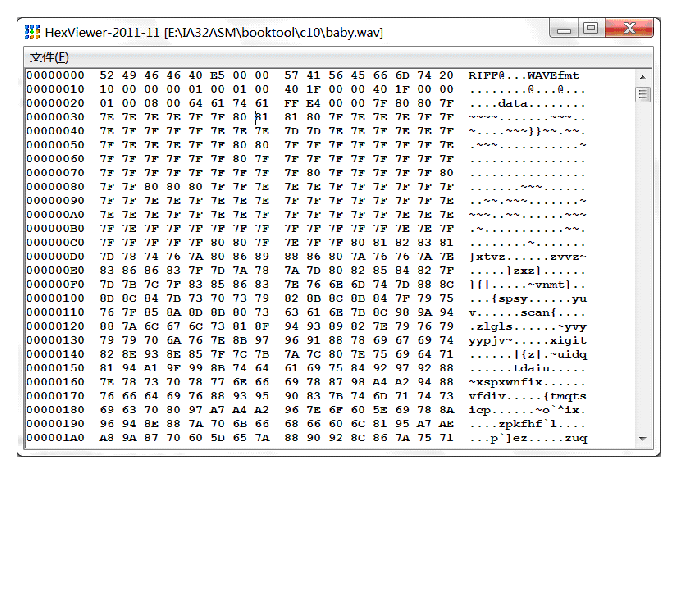
\includegraphics[width=\textwidth]{eps/10-8.bmp.eps}
\caption{以十六进制形式显示的baby.wav文件内容}\label{baby.wav}
\end{center}
\end{figure}
%图10-8  以十六进制形式显示的baby.wav文件内容

经仔细观察和分析可以知道, 这是一个8位、单声道、采样率为8000Hz的音频文件。你一定很好奇, 想知道是什么声音。好吧, 这是我女儿一岁时的笑声, 这段录音的长度只有7秒钟, 但是, 数据量却还是很大的, 有57KB。如果样本宽度是16位, 立体声, 采样率为44100Hz的话, 同样是录制7秒钟, 数据量会达到600KB。

怎么样, 看着这些数字, 你一定很难相信, 这居然就是声音?是的, 这就是数字化的声音。你可能会想到用其它波形文件来做实验, 这是可以的, 但SB-16针对不同的采样率和样本宽度有不同的编程方法, 请仔细阅读配书工具中提供的声霸卡硬件开发手册。注意, SB-16最高支持44100Hz的采样率, 所以一定要仔细, 只选择那些符合要求的文件。

前面所做的工作是关闭DMA通道1以便对其进行设置。现在, 代码清单10-1的第155~179行用于设置DMA缓冲区的起始地址和数据长度。DMA传送是自动进行的, 它需要一个起始地址是很自然的事。不过, 它毕竟不是处理器, 也没有逻辑地址的概念, 它要求的是一个物理地址, 也就是真实的地址。

缓冲区是由标号 voice\_{}data 指示的, 它们于数据段 data 内, 起始的偏移地址就是标号 voice\_{}data
在编译阶段的汇编地址。所以, 只需要在用户程序运行时, 把段寄存器 DS 的内容乘以 16, 再加上标号
voice\_{}data 的汇编地址就能得到该缓冲区的物理地址。

所以, 第155~160行, 首先取得段寄存器DS的内容, 乘以16, 结果的高16位在DX中 (仅低4位有效) , 低16位在AX中。接着, 加上偏移地址。注意adc指令, 它在两个大数相加时是必需的, 以前我们也这样用过。由于寄存器DX要用做端口号, 所以现在由BX:AX提供20位物理地址。

现在要做的是设置DMA控制器主片通道1的基准地址寄存器、当前地址寄存器、基准字数寄存器和当前字数寄存器。不过, 这些都是16位的寄存器, 而访问它们的端口都是8位的, 所以要分两次进行。每个DMA芯片都有一个公用的先后触发器 (或者叫字节指针触发器) , 用来控制写入次序。

82C37A主片的先后触发器口地址为0x0c, 通过向该端口写入一个任意值, 可以将它初始化到一个确定的状态。此后, 第一次向地址寄存器和字数寄存器写入时, 对应的是低字节;第二次写入时, 对应的是高字节。因此, 第162~163行, 向0x0c号端口写数值0以初始化写入顺序。

要设置82C37A主片通道1的基准地址寄存器和当前地址寄存器, 可以通过端口0x02。第165~168行, 写入前面计算机来的缓冲区物理地址, 分别是低8位和高8位。缓冲区的物理地址是20位, 位于BX:AX, 这里仅仅提供的是低16位, 还有高4位。毕竟, 系统总线的宽度是20位, 每次DMA传送时, 82C37A必须发出20位的物理地址, 而不是16位。

不过, 当前地址寄存器确实只有16位, 不足以形成20位地址。所以, 每个82C37A的DMA通道还各自有一个8位的页面寄存器, 使用它, 可以提供20位物理地址的高4位。

82C37A主片通道1的页面寄存器使用端口号0x83, 所以, 第162~163行, 将寄存器BL中的数值写入该端口 (仅低4位有效) 。

接下来设置82C37A主片通道1的基准字数寄存器和当前字数寄存器, 它们对应的端口号是0x03。第174~179行用于设置这两个寄存器。在我们这个特殊的例子中, 波形文件的大小是约57KB, 精确的数值可以用标号init\_{}msg的汇编地址减去voice\_{}data的汇编地址, 因为数据位于这两个标号之间。82C37A要求的数值是实际长度减一, 这是第176行所做的工作。

DMA传送有好几种方式, 分为单字节操作、数据块操作、请求操作和级联方式。单字节操作方式是, 先由外部设备进行DMA请求, 获得响应后, 82C371占用总线, 操作一个字节, 然后交还总线控制权给处理器。即使是有很多数据, 每操作一个字节, 都要按以上步骤进行。

表面上看起来, 这种操作方式不会很快。但事实上, 它依然是很快的, 毕竟用它来传送数据时, 不需要处理器中转。而且处理器每次接到总线请求时, 会立即在当前总线周期结束时让出总线。这是什么意思呢?当处理器接到DMA请求时, 它可能正在执行指令, 可能正在按指令的要求访问总线 (访问内存和I/O设备) 。这时, 它得先做完总线上的事, 不能半途而废。如果当时并未访问总线, 它可以立即让出总线控制权。总之, 它会果断地让出总线控制权, 而不用等到当前指令执行完毕。在乐观的情况下, 如果当前指令的操作不需要访问总线, 那么, 在让出总线控制权后, 处理器依然可以进行内部操作。单字节操作的好处是处理器会有很多“喘息”的机会来继续处理其它任务。

数据块操作方式是, 一旦DMA操作开始了, DMA控制器就一直占用总线, 直到操作完成。在此期间, 即使外部设备的DMA请求变得无效, 82C37A也一直占用总线, 暂停操作, 直至DMA请求变为有效。

请求操作的方式是, 是以否有DMA请求来决定, 如果有DMA请求, 则占用总线并进行DMA操作;当DMA请求无效或者操作完成时, 释放总线。
级联方式是为了对DMA进行扩展, 对多个82C37A芯片进行级联。

第181~182行, 用于设定82C37A的工作方式。可以设定每个通道的工作方式, 具体的做法是, 向主片或者从片的端口发送命令代码。主片上的端口号是0x0b;从片的端口号是0xd6。命令代码的格式如图 \ref{dma_name} 所示。据图可以知道, 当前设置的工作方式是:通道1, 读传送, 单字节操作方式, 地址递增, 自动预置。这里的术语大部分都在前面解释过了, 地址递增会使得每传送一个字节, 当前地址寄存器加一;自动预置使得当前字数寄存器的内容达到零时, 自动用基准寄存器的内容来填写相应的当前地址寄存器和当前字数寄存器。最后, 从存储器到外部设备的传送称为读传送;从外部设备到存储器的传送称为写传送。校验操作在DMA操作期间进行的不是数据传送, 而是对数据的正确性进行校验。
 
\begin{figure}
\begin{center}
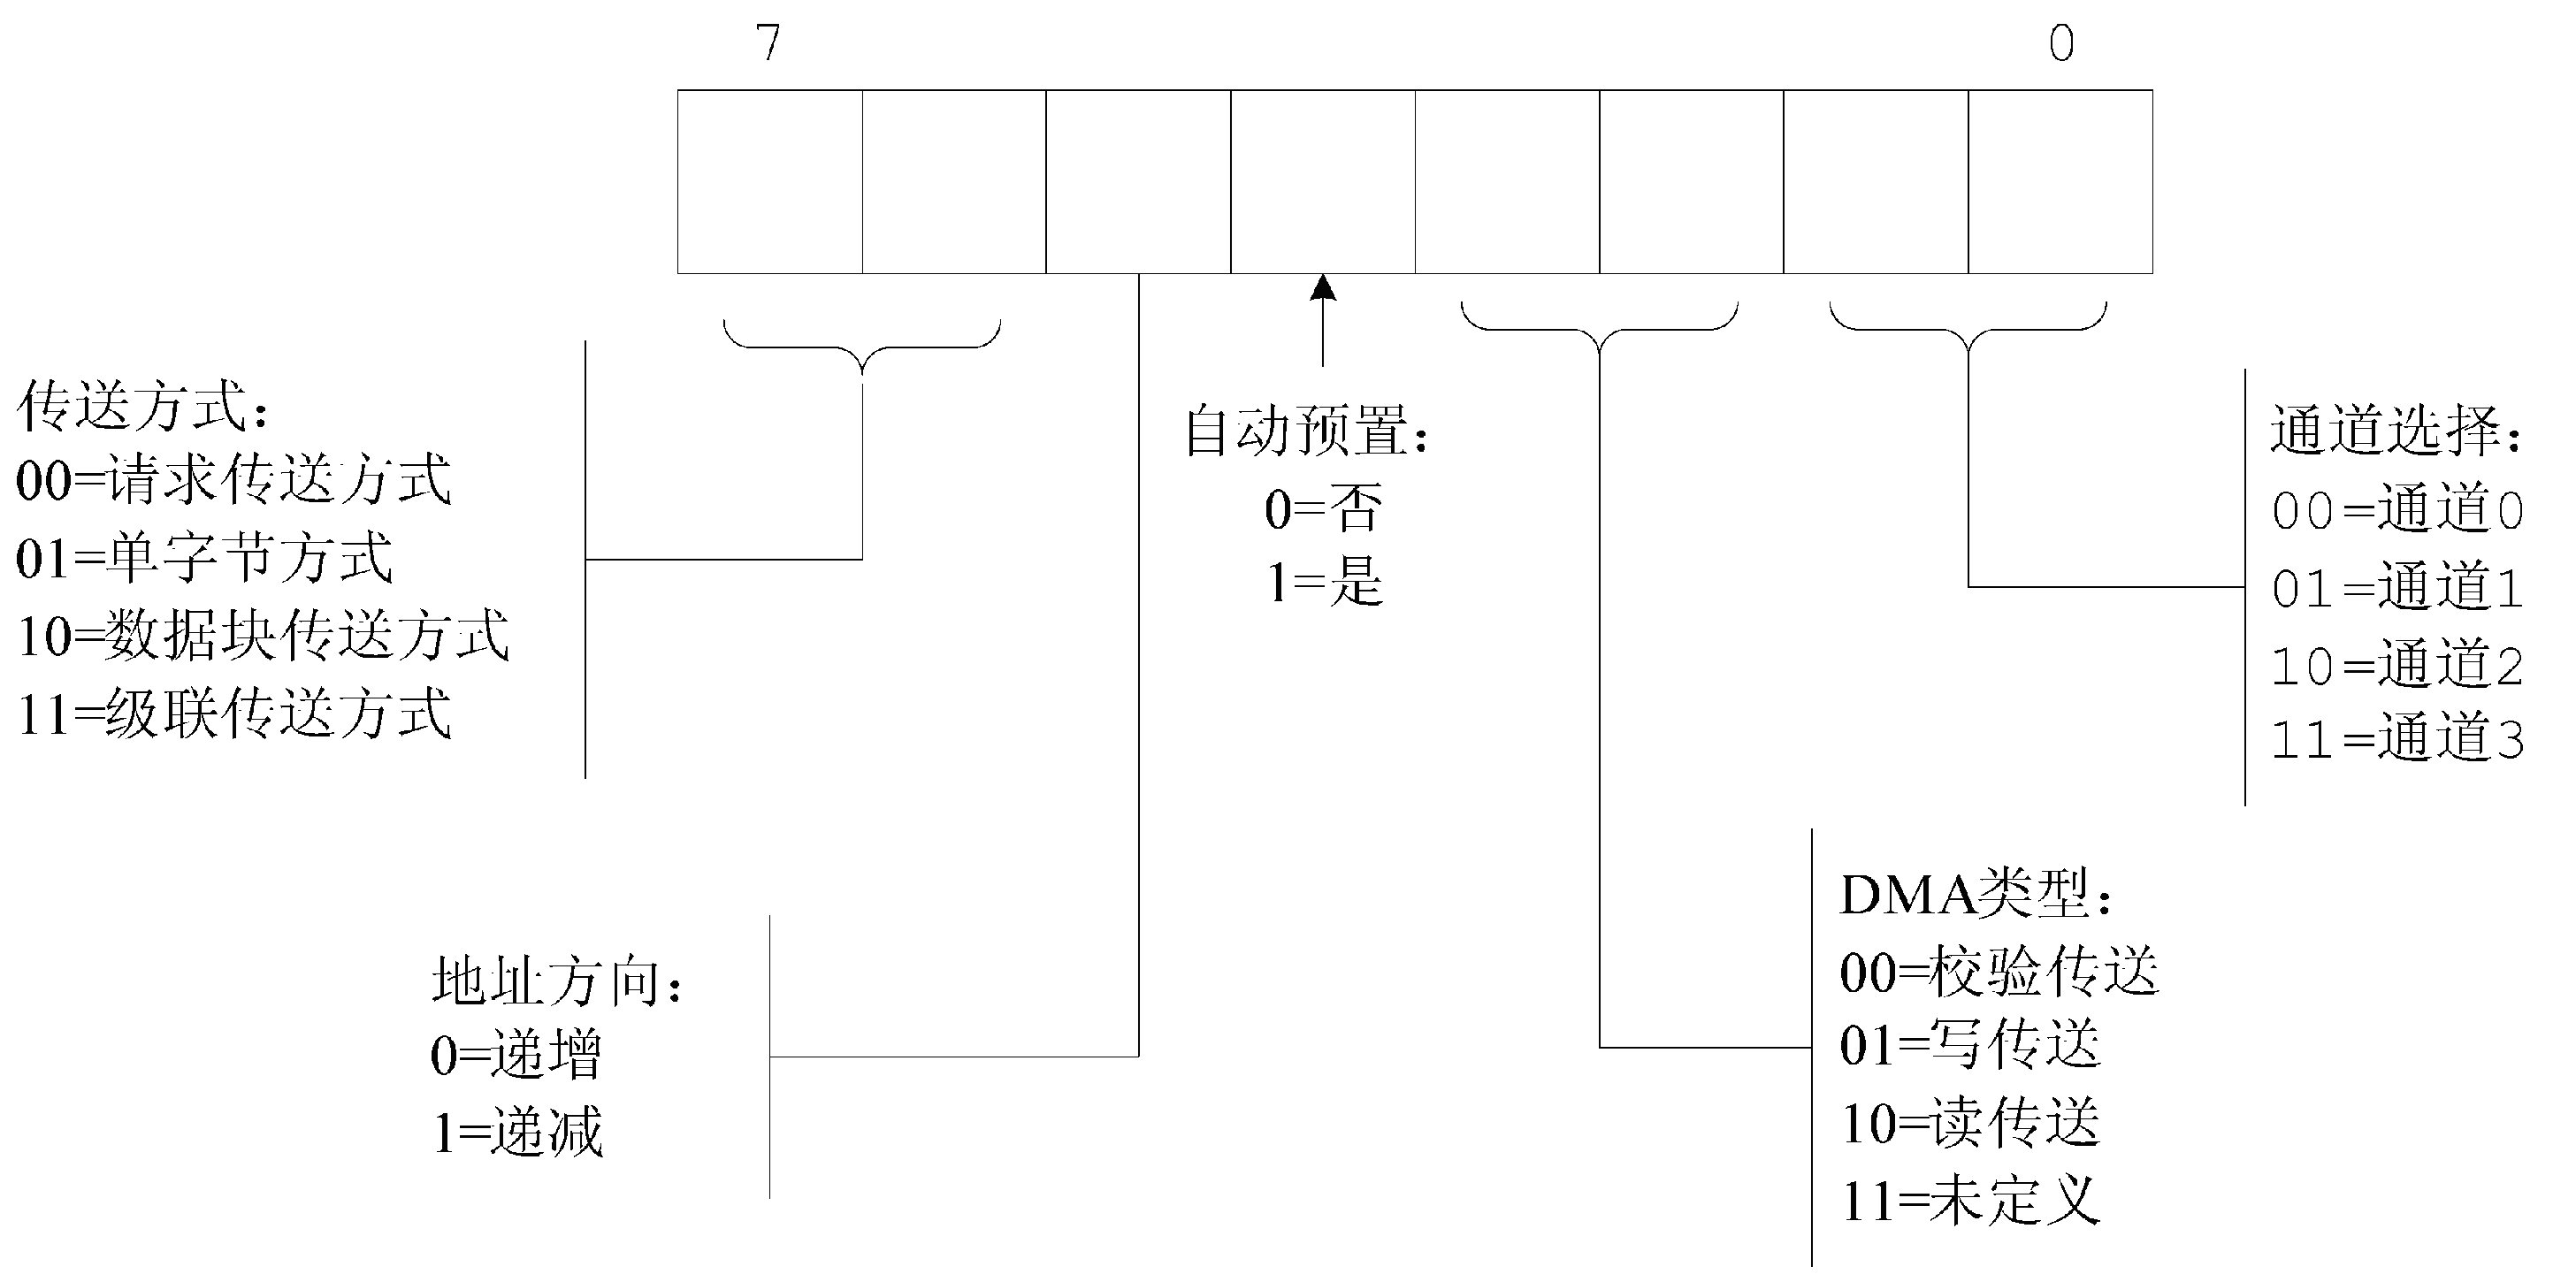
\includegraphics[width=\textwidth]{eps/10-9.bmp.eps}
\caption{DMA通道工作方式命令的格式}\label{dma_name}
\end{center}
\end{figure}
%图10-9  DMA通道工作方式命令的格式

最后, 第184~186行, 用于设置82C37A主片的屏蔽寄存器, 允许通道1接受DMA请求。

\subsection{启动音频播放 (xchg)}

接着初始化和设置声卡。SB-16有多种播放模式, 每种模式有不同的设置要求。鉴于本书的主题, 一一介绍可能会很困难。好吧, 不妨有针对性一些, 因为本书采用的波形文件是8位单声道, 采样率8000Hz, 所以, 在这里仅采用和介绍8位单声道自动初始化传输模式 (8 bit Mono Auto-initialize Transfer) 。

在这种模式下, DMA控制器也应当设置为自动预置状态, 每当指定数量的字节传送之后, 当前字数寄存器恢复为和基准字数寄存器一样。而对于声卡来说, 需要在播放前设置数据块的大小为DMA缓冲区的一半。回放开始后, 每次播放的数据量达到这个数值时,  声卡将会发出一个中断信号, 使程序可以继续用新的数据填充已回放的区域。

首先是设置声卡回放速率时间常量。SB-16给出的计算方法是

时间常量 = 65536 -  (256 000 000/ (声道数 × 采样率) ) 

第199~200行, 首先通过过程调用write\_{}dsp来向声卡的0x22c端口写入数值0x40, 表示准备写入回放速率时间常量。接着,  第190行, 用来计算实际的时间常量, 其数值是在程序编译期间计算的。声道数和采样率可以从波形文件的文件头中得到, 所以, 一般来说, 不应该在程序中采用这种硬性编码的方法, 这是一种非常不好的编程风格, 这么做唯一的原因是图个方便, 但希望读者们不要向我学习。
计算出来的数值是16位的, 在寄存器AX中, 但SB-16只使用其高8位。因此, 第191~192行, 将AH和AL中的内容互换, 然后将AL中的内容写入0x22c端口。

xchg是交换指令, 用于交换两个操作数的内容, 其格式为
\begin{verbatim}
xchg r8,m8
xchg r8,r8
xchg m8,r8
xchg r16,m16
xchg r16,r16
xchg m16,r16
\end{verbatim}
举个例子:
\begin{verbatim}
mov cx,0xf000
mov dx,0xcde0
xchg cx,dx
\end{verbatim}
以上指令执行后, 寄存器CX中的内容为0xcde0, DX中的内容为0xf000。
第199行, 通过调用过程write\_{}dsp来向0x22c端口写入命令字0x48, 这表示我们要写入数据块的长度。对于8位单声道音频来说, 数据块的长度是DMA缓冲区长度的一半减1。这样做的目的, 是允许声卡在播放到一半的时候, 发出一个中断, 以方便立即开始填充已回放的数据块, 避免声音中断。

第201行, 先将两个标号的汇编地址相减, 以得到缓冲区的长度;接着, 第202行, 将该长度右移一次, 这相当于将其除以2;第203行, 按声卡的要求, 将其减1。

第 204 行, 先通过调用过程 write\_{}dsp 来向 0x22c 端口写入数据块长度的低 8 位;
接着, 交换寄存器 AH 和 AL 的内容, 使 AL 中的内容变成数据块长度的高 8 位;
第 206 行, 通过调用过程 write\_{}dsp 来向 0x22c 端口写入高 8 位。

第209~210行, 通过调用过程write\_{}dsp来向0x22c端口写入命令字0xd1以打开扬声器。

第213~214行, 通过调用过程write\_{}dsp来向0x22c端口写入命令字0x1c, 以正式启动音频回放。

注意, 以上各个步骤所使用的命令字, 都是8位单声道自动初始化模式所专用的, 其它模式也有自己专用的命令字。8位立体声、16位单声道、16位立体声都是不同的。

如果你感兴趣, 可以阅读配书工具中提供的声霸卡硬件开发手册, 这是一个PDF文件。

最后, 第216~221行, 在显示了一个表明初始化结束, 声卡已经开发播放的消息后, 主程序使用处理器进入停机状态。但是, 中断和DMA系统是不会停止工作的, 声卡更不会知道这一切, 它只按自己的方式工作。

\subsection{音频回放中断处理}
一旦下达了命令字0x1c, 声卡就开始启动音频回放, 这个过程是独立于处理器的。当它播放的内容长度达到DMA缓冲区的一半时, 就会产生中断信号, 一般情况下, 中断号为5。

从代码清单10-1的第224行开始, 是中断处理过程。按规矩, 在中断处理过程的开始部分, 先将要用到的各个寄存器压栈保护。

在一个完备的音频回放中断处理过程中, 应当用声音数据填充已经播放过的那一半缓冲区。如果所有的数据都已经播放完了, 就发送命令使声卡退出自动初始化模式。注意, 本章的例子符合后一种情况。因为程序中包含了所有的音频数据, 当中断发生时, 不需要填充数据, 直接退出回放即可。

如代码清单10-1的第230~231行所示, 退出自动初始化模式的方法是向0x22c端口写命令字0xda。你可能会想, 一旦发出此命令, 声卡岂不会立即停止工作?此时才播放了一半的数据, 另一半数据岂不是无法继续播放了?

不用担心, 中断发生时, 声卡正在播放缓冲区的后半部分。当声卡接到此命令时, 它不会立即停止工作, 只有在当前数据块播放结束之后, 它才会真正退出自动初始化模式。

第234~235行, 调用过程write\_{}dsp来向声卡发送关闭扬声器的命令0xd3。

第237~241行用地在屏幕上显示一条消息, 表明声音的回放已经结束了。

第243~244行, 在正常的声卡中断处理过程中, 应当读一下0x22f端口, 作为对声卡中断的应答。

第247~248行, 和往常一样, 在中断处理过程结束之前, 向中断控制器发送中断结束应答信号。因为声卡连接在8259主片上, 故仅需要向主片发送。

\subsection{程序的编译和运行}

如图 \ref{src_code} 所示, 请首先确保本章的源程序文件 c10.asm 和 baby.wav
是在一起的, 位于同一下文件夹下。然后, 编译源程序以生成c10.bin文件。
 
\begin{figure}
\begin{center}
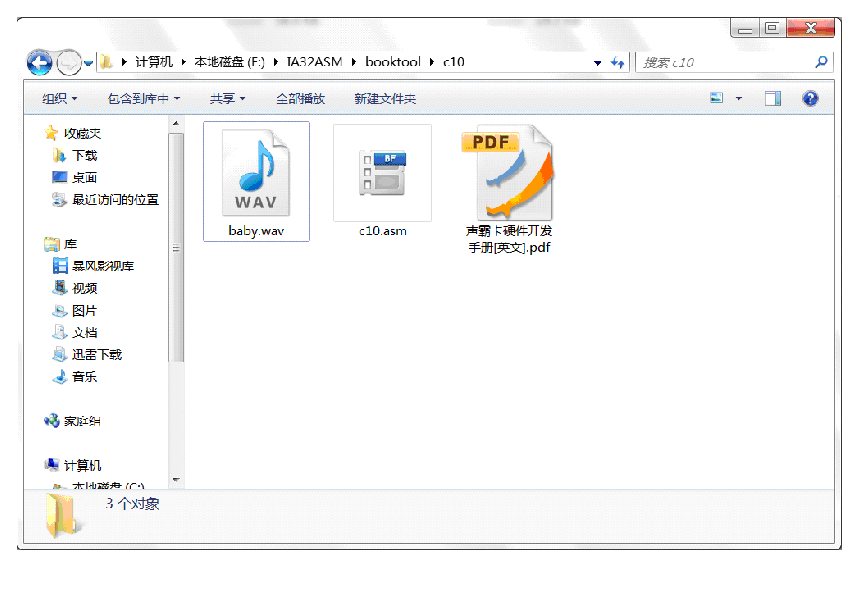
\includegraphics[width=\textwidth]{eps/10-10.bmp.eps}
\caption{本章配套的源程序文件和波形文件}\label{src_code}
\end{center}
\end{figure}
%图10-10  本章配套的源程序文件和波形文件

首先将编译后的二进制文件写入虚拟硬盘, 从逻辑扇区100开始。然后, 打开音箱电源, 稍微将音量放大一点, 启动虚拟机, 观察屏幕显示, 并聆听扬声器的发出的声音。如果一切正常, 虚拟机运行时的屏幕如图 \ref{result} 所示。
 
\begin{figure}
\begin{center}
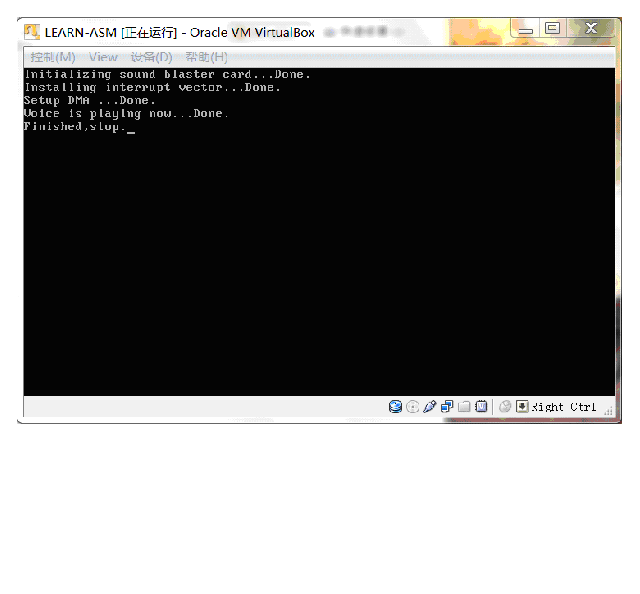
\includegraphics[width=\textwidth]{eps/10-11.bmp.eps}
\caption{本章程序运行结果}\label{result}
\end{center}
\end{figure}
%图10-11  本章程序运行结果

\subsection{本章习题}
\begin{enumerate}
\item 如果可能的话, 修改本章的源代码, 使得不用硬性编码, 而是从波形文件的文件头中取得参数, 并计算播放速度的时间常数。
\end{enumerate}




\newpage
\end{CJK}
\end{document}
